%%%%%%%%%%%%%%%%%%%%%%%%%%%%%%%%%%%%%%%%%%%%%%%%%%%%%%%%%%%%
% 3.3 VECTOR GEOMETRY
% The Composition of Advanced Mathematics
%%%%%%%%%%%%%%%%%%%%%%%%%%%%%%%%%%%%%%%%%%%%%%%%%%%%%%%%%%%%

\section{Vector Geometry}
\label{sec:vector-geometry}

\prerequisite{
Analytic / Coordinate Geometry from
\cref{sec:analytic-coordinate-geometry},
Euclidean Geometry from \cref{sec:euclidean-geometry},
and Linear Algebra from \cref{sec:linear-algebra}.
}

\learningobjectives{
By the end of this section, the reader should be able to:
\begin{itemize}
    \item distinguish vectors from points and scalars;
    \item represent vectors geometrically and in component form;
    \item compute vector magnitude and direction;
    \item add, subtract, and scale vectors;
    \item construct vectors between points;
    \item normalize vectors and identify unit vectors;
    \item use the dot product to determine angles and orthogonality;
    \item compute scalar and vector projections;
    \item interpret the Cauchy--Schwarz and triangle inequalities geometrically;
    \item use the cross product in three-dimensional geometry;
    \item compute areas using cross products and determinants;
    \item describe lines and planes using vector equations;
    \item compute distances involving points, lines, and planes;
    \item interpret geometric objects through vector methods;
    \item connect vector geometry with linear algebra, calculus,
    differential geometry, and mathematical physics.
\end{itemize}
}

%%%%%%%%%%%%%%%%%%%%%%%%%%%%%%%%%%%%%%%%%%%%%%%%%%%%%%%%%%%%
\subsection{From Coordinates to Vectors}
\label{subsec:coordinates-to-vectors}
%%%%%%%%%%%%%%%%%%%%%%%%%%%%%%%%%%%%%%%%%%%%%%%%%%%%%%%%%%%%

Coordinate geometry describes position using ordered coordinates.

Vector geometry introduces objects that describe both \emph{magnitude} and
\emph{direction}.

For example, the points

\[ A=(1,2),\qquad B=(5,5) \]

determine the displacement

\[ (5-1,5-2)=(4,3). \]

Rather than describing where a point is located, this pair describes how to
move from one point to another.

That directed displacement is a vector.

\begin{definitionbox}{Vector}
A \emph{vector} is a mathematical object possessing magnitude and direction.

In Cartesian coordinates, a vector in \(\R^n\) may be represented by an
ordered list of components.
\end{definitionbox}

%%%%%%%%%%%%%%%%%%%%%%%%%%%%%%%%%%%%%%%%%%%%%%%%%%%%%%%%%%%%
\subsection{Vector Notation}
\label{subsec:vector-notation}
%%%%%%%%%%%%%%%%%%%%%%%%%%%%%%%%%%%%%%%%%%%%%%%%%%%%%%%%%%%%

Vectors are commonly written using bold symbols or arrows:

\[ \mathbf{v},\qquad \vec{v}. \]

In this text, bold notation will usually be used.

A vector in the plane may be written

\[ \mathbf{v}=\langle v_1,v_2\rangle. \]

The angle brackets

\[ \langle\,\cdot\,\rangle \]

are read ``angle brackets.''

Thus

\[ \langle 3,-2\rangle \]

is read ``the vector three, negative two.''

In three dimensions,

\[ \mathbf{v}=\langle v_1,v_2,v_3\rangle. \]

More generally,

\[ \mathbf{v}=\langle v_1,\ldots,v_n\rangle\in\R^n. \]

%%%%%%%%%%%%%%%%%%%%%%%%%%%%%%%%%%%%%%%%%%%%%%%%%%%%%%%%%%%%
\subsection{Vectors and Points}
\label{subsec:vectors-and-points}
%%%%%%%%%%%%%%%%%%%%%%%%%%%%%%%%%%%%%%%%%%%%%%%%%%%%%%%%%%%%

Points and vectors may use similar coordinate lists, but conceptually they
play different roles.

A point

\[ P=(3,2) \]

describes a \emph{location}.

A vector

\[ \mathbf{v}=\langle3,2\rangle \]

describes a \emph{displacement} or directed quantity.

In Euclidean coordinate spaces, a point can be associated with its
\emph{position vector} from the origin.

For

\[ P=(3,2), \]

the position vector is

\[ \overrightarrow{OP}=\langle3,2\rangle. \]

This identification is convenient, but the conceptual distinction between
points and vectors remains important.

%%%%%%%%%%%%%%%%%%%%%%%%%%%%%%%%%%%%%%%%%%%%%%%%%%%%%%%%%%%%
\subsection{Geometric Representation of a Vector}
\label{subsec:geometric-vector-representation}
%%%%%%%%%%%%%%%%%%%%%%%%%%%%%%%%%%%%%%%%%%%%%%%%%%%%%%%%%%%%

A vector is represented geometrically by a directed line segment.

\begin{centereddiagram}
\begin{tikzpicture}[scale=0.85]
\draw[->] (-1,0)--(5,0) node[right] {\(x\)};
\draw[->] (0,-1)--(0,4) node[above] {\(y\)};

\draw[-{Latex[length=3mm]},very thick] (0.5,0.5)--(4,3);
\node[above left] at (2.5,2) {\(\mathbf{v}\)};

\fill (0.5,0.5) circle (2pt);
\fill (4,3) circle (2pt);

\node[below] at (0.5,0.5) {tail};
\node[above right] at (4,3) {head};
\end{tikzpicture}
\end{centereddiagram}

The starting point is the \emph{tail}.

The ending point is the \emph{head}.

The vector points from tail to head.

%%%%%%%%%%%%%%%%%%%%%%%%%%%%%%%%%%%%%%%%%%%%%%%%%%%%%%%%%%%%
\subsection{Free Vectors}
\label{subsec:free-vectors}
%%%%%%%%%%%%%%%%%%%%%%%%%%%%%%%%%%%%%%%%%%%%%%%%%%%%%%%%%%%%

In elementary Euclidean vector geometry, a vector is usually treated as a
\emph{free vector}.

This means the vector can be translated without changing it, provided its
magnitude and direction remain unchanged.

\begin{centereddiagram}
\begin{tikzpicture}[scale=0.8]
\draw[-{Latex[length=3mm]},thick] (0,0)--(2.5,1.5);
\draw[-{Latex[length=3mm]},thick] (1,2)--(3.5,3.5);
\draw[-{Latex[length=3mm]},thick] (4,0.5)--(6.5,2);

\node at (1.2,-0.5) {\(\mathbf{v}\)};
\node at (2.3,1.5) {\(\mathbf{v}\)};
\node at (5.5,0.6) {\(\mathbf{v}\)};
\end{tikzpicture}
\end{centereddiagram}

All three arrows represent the same free vector.

%%%%%%%%%%%%%%%%%%%%%%%%%%%%%%%%%%%%%%%%%%%%%%%%%%%%%%%%%%%%
\subsection{Vectors Between Points}
\label{subsec:vectors-between-points}
%%%%%%%%%%%%%%%%%%%%%%%%%%%%%%%%%%%%%%%%%%%%%%%%%%%%%%%%%%%%

Let

\[ A=(x_1,y_1),\qquad B=(x_2,y_2). \]

The vector pointing from \(A\) to \(B\) is

\[ \boxed{\overrightarrow{AB}=\langle x_2-x_1,y_2-y_1\rangle.} \]

The notation \(\overrightarrow{AB}\) is read ``vector \(AB\),'' or
``the vector from \(A\) to \(B\).''

In three dimensions,

\[
A=(x_1,y_1,z_1),\qquad
B=(x_2,y_2,z_2),
\]

so

\[
\boxed{
\overrightarrow{AB}
=
\langle
x_2-x_1,
y_2-y_1,
z_2-z_1
\rangle.
}
\]

The order matters:

\[ \overrightarrow{BA}=-\overrightarrow{AB}. \]

%%%%%%%%%%%%%%%%%%%%%%%%%%%%%%%%%%%%%%%%%%%%%%%%%%%%%%%%%%%%
\subsection{Worked Example: Vector Between Points}
\label{subsec:worked-vector-between-points}
%%%%%%%%%%%%%%%%%%%%%%%%%%%%%%%%%%%%%%%%%%%%%%%%%%%%%%%%%%%%

\begin{workedexamplebox}{Finding a Vector Between Two Points}

Let

\[ A=(-2,3),\qquad B=(5,7). \]

Find \(\overrightarrow{AB}\).

\begin{tabularx}{\textwidth}{@{}>{\raggedright\arraybackslash}p{0.43\textwidth}X@{}}
Subtract initial coordinates from terminal coordinates. &
\(\overrightarrow{AB}=\langle5-(-2),7-3\rangle\)\\
Simplify. &
\(\overrightarrow{AB}=\langle7,4\rangle\)
\end{tabularx}

\begin{answerbox}
\[ \boxed{\overrightarrow{AB}=\langle7,4\rangle} \]
\end{answerbox}
\end{workedexamplebox}

%%%%%%%%%%%%%%%%%%%%%%%%%%%%%%%%%%%%%%%%%%%%%%%%%%%%%%%%%%%%
\subsection{Equality of Vectors}
\label{subsec:equality-of-vectors}
%%%%%%%%%%%%%%%%%%%%%%%%%%%%%%%%%%%%%%%%%%%%%%%%%%%%%%%%%%%%

Two vectors are equal when their corresponding components are equal.

For

\[
\mathbf{u}=\langle u_1,u_2\rangle,\qquad
\mathbf{v}=\langle v_1,v_2\rangle,
\]

we have

\[
\boxed{
\mathbf{u}=\mathbf{v}
\iff
u_1=v_1
\text{ and }
u_2=v_2.
}
\]

Geometrically, equal free vectors have the same magnitude and direction.

%%%%%%%%%%%%%%%%%%%%%%%%%%%%%%%%%%%%%%%%%%%%%%%%%%%%%%%%%%%%
\subsection{The Zero Vector}
\label{subsec:zero-vector-geometry}
%%%%%%%%%%%%%%%%%%%%%%%%%%%%%%%%%%%%%%%%%%%%%%%%%%%%%%%%%%%%

\begin{definitionbox}{Zero Vector}
The \emph{zero vector} is the vector whose components are all zero:

\[ \boxed{\mathbf{0}=\langle0,\ldots,0\rangle.} \]
\end{definitionbox}

The zero vector has magnitude zero.

It does not have a uniquely defined direction.

%%%%%%%%%%%%%%%%%%%%%%%%%%%%%%%%%%%%%%%%%%%%%%%%%%%%%%%%%%%%
\subsection{Vector Addition}
\label{subsec:vector-addition-geometry}
%%%%%%%%%%%%%%%%%%%%%%%%%%%%%%%%%%%%%%%%%%%%%%%%%%%%%%%%%%%%

Vectors are added componentwise.

If

\[
\mathbf{u}=\langle u_1,u_2\rangle,\qquad
\mathbf{v}=\langle v_1,v_2\rangle,
\]

then

\[ \boxed{\mathbf{u}+\mathbf{v}=\langle u_1+v_1,u_2+v_2\rangle.} \]

In three dimensions,

\[
\boxed{
\langle u_1,u_2,u_3\rangle+
\langle v_1,v_2,v_3\rangle
=
\langle u_1+v_1,u_2+v_2,u_3+v_3\rangle.
}
\]

%%%%%%%%%%%%%%%%%%%%%%%%%%%%%%%%%%%%%%%%%%%%%%%%%%%%%%%%%%%%
\subsection{Head-to-Tail Addition}
\label{subsec:head-tail-addition}
%%%%%%%%%%%%%%%%%%%%%%%%%%%%%%%%%%%%%%%%%%%%%%%%%%%%%%%%%%%%

Geometrically, vector addition can be performed by placing the tail of the
second vector at the head of the first.

\begin{centereddiagram}
\begin{tikzpicture}[scale=0.85]
\coordinate (O) at (0,0);
\coordinate (A) at (3,1);
\coordinate (B) at (4.5,3);

\draw[-{Latex[length=3mm]},thick] (O)--(A);
\draw[-{Latex[length=3mm]},thick] (A)--(B);
\draw[-{Latex[length=3mm]},very thick] (O)--(B);

\node[below] at (1.5,0.5) {\(\mathbf{u}\)};
\node[right] at (3.8,2) {\(\mathbf{v}\)};
\node[above left] at (2.2,1.7) {\(\mathbf{u}+\mathbf{v}\)};
\end{tikzpicture}
\end{centereddiagram}

The resulting vector runs from the original tail to the final head.

%%%%%%%%%%%%%%%%%%%%%%%%%%%%%%%%%%%%%%%%%%%%%%%%%%%%%%%%%%%%
\subsection{The Parallelogram Law}
\label{subsec:parallelogram-law-vectors}
%%%%%%%%%%%%%%%%%%%%%%%%%%%%%%%%%%%%%%%%%%%%%%%%%%%%%%%%%%%%

If \(\mathbf{u}\) and \(\mathbf{v}\) begin at the same point, their sum is
the diagonal of the parallelogram formed by the two vectors.

\begin{centereddiagram}
\begin{tikzpicture}[scale=0.85]
\coordinate (O) at (0,0);
\coordinate (U) at (3,0.7);
\coordinate (V) at (1.2,2.4);
\coordinate (S) at (4.2,3.1);

\draw[-{Latex[length=3mm]},thick] (O)--(U);
\draw[-{Latex[length=3mm]},thick] (O)--(V);
\draw[dashed] (U)--(S);
\draw[dashed] (V)--(S);
\draw[-{Latex[length=3mm]},very thick] (O)--(S);

\node[below] at (1.5,0.35) {\(\mathbf{u}\)};
\node[left] at (0.6,1.2) {\(\mathbf{v}\)};
\node[above left] at (2.3,1.8) {\(\mathbf{u}+\mathbf{v}\)};
\end{tikzpicture}
\end{centereddiagram}

%%%%%%%%%%%%%%%%%%%%%%%%%%%%%%%%%%%%%%%%%%%%%%%%%%%%%%%%%%%%
\subsection{Vector Subtraction}
\label{subsec:vector-subtraction-geometry}
%%%%%%%%%%%%%%%%%%%%%%%%%%%%%%%%%%%%%%%%%%%%%%%%%%%%%%%%%%%%

Vector subtraction is defined by adding the opposite vector:

\[ \boxed{\mathbf{u}-\mathbf{v}=\mathbf{u}+(-\mathbf{v}).} \]

Componentwise,

\[
\boxed{
\mathbf{u}-\mathbf{v}
=
\langle
u_1-v_1,
u_2-v_2
\rangle.
}
\]

The vector \(-\mathbf{v}\) has the same magnitude as \(\mathbf{v}\) but
points in the opposite direction.

%%%%%%%%%%%%%%%%%%%%%%%%%%%%%%%%%%%%%%%%%%%%%%%%%%%%%%%%%%%%
\subsection{Scalar Multiplication}
\label{subsec:scalar-multiplication-geometry}
%%%%%%%%%%%%%%%%%%%%%%%%%%%%%%%%%%%%%%%%%%%%%%%%%%%%%%%%%%%%

A real number used to multiply a vector is called a \emph{scalar}.

If \(c\in\R\), then

\[
\boxed{
c\mathbf{v}
=
\langle
cv_1,\ldots,cv_n
\rangle.
}
\]

Geometrically:

\begin{itemize}
    \item if \(c>1\), the vector is stretched;
    \item if \(0<c<1\), the vector is shortened;
    \item if \(c<0\), the direction is reversed and the magnitude is scaled;
    \item if \(c=0\), the result is \(\mathbf{0}\).
\end{itemize}

%%%%%%%%%%%%%%%%%%%%%%%%%%%%%%%%%%%%%%%%%%%%%%%%%%%%%%%%%%%%
\subsection{Magnitude of a Vector}
\label{subsec:vector-magnitude}
%%%%%%%%%%%%%%%%%%%%%%%%%%%%%%%%%%%%%%%%%%%%%%%%%%%%%%%%%%%%

The length of a vector is called its \emph{magnitude} or \emph{norm}.

\begin{definitionbox}{Euclidean Norm}
For

\[ \mathbf{v}=\langle v_1,\ldots,v_n\rangle, \]

the Euclidean norm is

\[ \boxed{\|\mathbf{v}\|=\sqrt{v_1^2+\cdots+v_n^2}.} \]
\end{definitionbox}

The notation

\[ \|\mathbf{v}\| \]

is read ``the norm of \(\mathbf{v}\)'' or ``the magnitude of
\(\mathbf{v}\).''

In \(\R^2\),

\[ \|\mathbf{v}\|=\sqrt{v_1^2+v_2^2}. \]

In \(\R^3\),

\[ \|\mathbf{v}\|=\sqrt{v_1^2+v_2^2+v_3^2}. \]

%%%%%%%%%%%%%%%%%%%%%%%%%%%%%%%%%%%%%%%%%%%%%%%%%%%%%%%%%%%%
\subsection{Magnitude and Distance}
\label{subsec:magnitude-and-distance}
%%%%%%%%%%%%%%%%%%%%%%%%%%%%%%%%%%%%%%%%%%%%%%%%%%%%%%%%%%%%

For points \(A\) and \(B\),

\[ \overrightarrow{AB}=B-A. \]

Therefore

\[
\boxed{
d(A,B)=\|\overrightarrow{AB}\|.
}
\]

This shows that the coordinate distance formula is simply the magnitude of
the displacement vector between two points.

%%%%%%%%%%%%%%%%%%%%%%%%%%%%%%%%%%%%%%%%%%%%%%%%%%%%%%%%%%%%
\subsection{Worked Example: Vector Magnitude}
\label{subsec:worked-vector-magnitude}
%%%%%%%%%%%%%%%%%%%%%%%%%%%%%%%%%%%%%%%%%%%%%%%%%%%%%%%%%%%%

\begin{workedexamplebox}{Finding Vector Magnitude}

Find the magnitude of

\[ \mathbf{v}=\langle3,-4,12\rangle. \]

\begin{tabularx}{\textwidth}{@{}>{\raggedright\arraybackslash}p{0.43\textwidth}X@{}}
Use the norm formula. &
\(\|\mathbf{v}\|=\sqrt{3^2+(-4)^2+12^2}\)\\
Square the components. &
\(\|\mathbf{v}\|=\sqrt{9+16+144}\)\\
Simplify. &
\(\|\mathbf{v}\|=\sqrt{169}=13\)
\end{tabularx}

\begin{answerbox}
\[ \boxed{\|\mathbf{v}\|=13} \]
\end{answerbox}
\end{workedexamplebox}

%%%%%%%%%%%%%%%%%%%%%%%%%%%%%%%%%%%%%%%%%%%%%%%%%%%%%%%%%%%%
\subsection{Properties of the Euclidean Norm}
\label{subsec:euclidean-norm-properties}
%%%%%%%%%%%%%%%%%%%%%%%%%%%%%%%%%%%%%%%%%%%%%%%%%%%%%%%%%%%%

For vectors \(\mathbf{u},\mathbf{v}\) and scalar \(c\),

\[
\|\mathbf{v}\|\geq0,
\]

and

\[ \|\mathbf{v}\|=0\iff\mathbf{v}=\mathbf{0}. \]

Also,

\[ \boxed{\|c\mathbf{v}\|=|c|\,\|\mathbf{v}\|.} \]

A fundamental inequality is

\[ \boxed{\|\mathbf{u}+\mathbf{v}\|\leq\|\mathbf{u}\|+\|\mathbf{v}\|.} \]

This is the \emph{triangle inequality}.

%%%%%%%%%%%%%%%%%%%%%%%%%%%%%%%%%%%%%%%%%%%%%%%%%%%%%%%%%%%%
\subsection{Triangle Inequality}
\label{subsec:vector-triangle-inequality}
%%%%%%%%%%%%%%%%%%%%%%%%%%%%%%%%%%%%%%%%%%%%%%%%%%%%%%%%%%%%

The triangle inequality has a direct geometric meaning.

Traveling directly from one point to another is no longer than traveling
through an intermediate point.

\begin{centereddiagram}
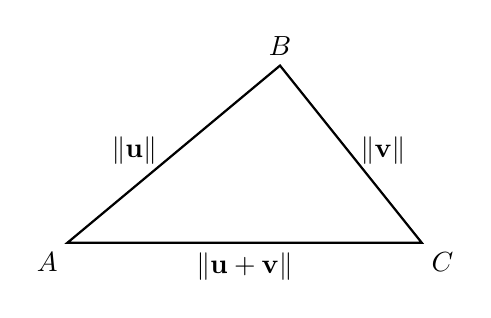
\begin{tikzpicture}[scale=0.9]
\coordinate (A) at (0,0);
\coordinate (B) at (3,2.5);
\coordinate (C) at (5,0);

\draw[thick] (A)--(B)--(C)--cycle;

\node[below left] at (A) {\(A\)};
\node[above] at (B) {\(B\)};
\node[below right] at (C) {\(C\)};

\node[left] at (1.4,1.3) {\(\|\mathbf{u}\|\)};
\node[right] at (4,1.3) {\(\|\mathbf{v}\|\)};
\node[below] at (2.5,0) {\(\|\mathbf{u}+\mathbf{v}\|\)};
\end{tikzpicture}
\end{centereddiagram}

Thus

\[ \|\mathbf{u}+\mathbf{v}\|\leq\|\mathbf{u}\|+\|\mathbf{v}\|. \]

Equality occurs when the vectors point in the same direction, including
degenerate zero-vector cases.

%%%%%%%%%%%%%%%%%%%%%%%%%%%%%%%%%%%%%%%%%%%%%%%%%%%%%%%%%%%%
\subsection{Unit Vectors}
\label{subsec:unit-vectors}
%%%%%%%%%%%%%%%%%%%%%%%%%%%%%%%%%%%%%%%%%%%%%%%%%%%%%%%%%%%%

\begin{definitionbox}{Unit Vector}
A \emph{unit vector} is a vector having magnitude \(1\).
\end{definitionbox}

Thus

\[ \|\mathbf{u}\|=1. \]

In \(\R^2\), the standard coordinate unit vectors are

\[ \boxed{\mathbf{i}=\langle1,0\rangle,\qquad\mathbf{j}=\langle0,1\rangle.} \]

In \(\R^3\),

\[
\boxed{
\mathbf{i}=\langle1,0,0\rangle,\quad
\mathbf{j}=\langle0,1,0\rangle,\quad
\mathbf{k}=\langle0,0,1\rangle.
}
\]

These point along the positive coordinate axes.

%%%%%%%%%%%%%%%%%%%%%%%%%%%%%%%%%%%%%%%%%%%%%%%%%%%%%%%%%%%%
\subsection{Component Representation Using Unit Vectors}
\label{subsec:unit-vector-components}
%%%%%%%%%%%%%%%%%%%%%%%%%%%%%%%%%%%%%%%%%%%%%%%%%%%%%%%%%%%%

A vector

\[ \mathbf{v}=\langle a,b\rangle \]

may be written

\[ \boxed{\mathbf{v}=a\mathbf{i}+b\mathbf{j}.} \]

In three dimensions,

\[ \boxed{\mathbf{v}=a\mathbf{i}+b\mathbf{j}+c\mathbf{k}.} \]

This notation is especially common in physics and engineering.

%%%%%%%%%%%%%%%%%%%%%%%%%%%%%%%%%%%%%%%%%%%%%%%%%%%%%%%%%%%%
\subsection{Normalization}
\label{subsec:vector-normalization}
%%%%%%%%%%%%%%%%%%%%%%%%%%%%%%%%%%%%%%%%%%%%%%%%%%%%%%%%%%%%

Any nonzero vector can be converted into a unit vector pointing in the same
direction.

\begin{definitionbox}{Normalization}
For \(\mathbf{v}\neq\mathbf{0}\), the normalized vector is

\[ \boxed{\widehat{\mathbf{v}}=\frac{\mathbf{v}}{\|\mathbf{v}\|}.} \]
\end{definitionbox}

The symbol

\[ \widehat{\mathbf{v}} \]

is read ``v hat.''

It commonly denotes a unit vector in the direction of \(\mathbf{v}\).

Indeed,

\[
\left\|
\frac{\mathbf{v}}{\|\mathbf{v}\|}
\right\|
=
1.
\]

%%%%%%%%%%%%%%%%%%%%%%%%%%%%%%%%%%%%%%%%%%%%%%%%%%%%%%%%%%%%
\subsection{Worked Example: Unit Vector}
\label{subsec:worked-unit-vector}
%%%%%%%%%%%%%%%%%%%%%%%%%%%%%%%%%%%%%%%%%%%%%%%%%%%%%%%%%%%%

\begin{workedexamplebox}{Finding a Unit Vector}

Find a unit vector in the direction of

\[ \mathbf{v}=\langle3,4\rangle. \]

\begin{tabularx}{\textwidth}{@{}>{\raggedright\arraybackslash}p{0.43\textwidth}X@{}}
Find the magnitude. &
\(\|\mathbf{v}\|=\sqrt{3^2+4^2}=5\)\\
Divide by the magnitude. &
\(\widehat{\mathbf{v}}=\frac15\langle3,4\rangle\)\\
Simplify. &
\(\widehat{\mathbf{v}}=\left\langle\frac35,\frac45\right\rangle\)
\end{tabularx}

\begin{answerbox}
\[ \boxed{\widehat{\mathbf{v}}=\left\langle\frac35,\frac45\right\rangle} \]
\end{answerbox}
\end{workedexamplebox}

%%%%%%%%%%%%%%%%%%%%%%%%%%%%%%%%%%%%%%%%%%%%%%%%%%%%%%%%%%%%
\subsection{Direction Angles in the Plane}
\label{subsec:vector-direction-angle}
%%%%%%%%%%%%%%%%%%%%%%%%%%%%%%%%%%%%%%%%%%%%%%%%%%%%%%%%%%%%

For a nonzero vector

\[ \mathbf{v}=\langle a,b\rangle, \]

its direction angle \(\theta\) is the angle measured counterclockwise from
the positive \(x\)-axis.

Then

\[ \boxed{a=\|\mathbf{v}\|\cos\theta,\qquad b=\|\mathbf{v}\|\sin\theta.} \]

Hence

\[
\boxed{
\mathbf{v}
=
\|\mathbf{v}\|
\langle\cos\theta,\sin\theta\rangle.
}
\]

When \(a\neq0\),

\[ \tan\theta=\frac ba, \]

but the quadrant must be considered when recovering \(\theta\).

%%%%%%%%%%%%%%%%%%%%%%%%%%%%%%%%%%%%%%%%%%%%%%%%%%%%%%%%%%%%
\subsection{The Dot Product}
\label{subsec:dot-product-geometry}
%%%%%%%%%%%%%%%%%%%%%%%%%%%%%%%%%%%%%%%%%%%%%%%%%%%%%%%%%%%%

The dot product combines two vectors to produce a scalar.

\begin{definitionbox}{Dot Product}
For

\[
\mathbf{u}=\langle u_1,\ldots,u_n\rangle,\qquad
\mathbf{v}=\langle v_1,\ldots,v_n\rangle,
\]

their dot product is

\[ \boxed{\mathbf{u}\cdot\mathbf{v}=u_1v_1+\cdots+u_nv_n.} \]
\end{definitionbox}

The centered dot

\[ \cdot \]

is read ``dot.''

Thus

\[ \mathbf{u}\cdot\mathbf{v} \]

is read ``u dot v.''

%%%%%%%%%%%%%%%%%%%%%%%%%%%%%%%%%%%%%%%%%%%%%%%%%%%%%%%%%%%%
\subsection{Worked Example: Dot Product}
\label{subsec:worked-dot-product}
%%%%%%%%%%%%%%%%%%%%%%%%%%%%%%%%%%%%%%%%%%%%%%%%%%%%%%%%%%%%

\begin{workedexamplebox}{Computing a Dot Product}

Let

\[ \mathbf{u}=\langle2,-1,3\rangle,\qquad
\mathbf{v}=\langle4,5,-2\rangle. \]

\begin{tabularx}{\textwidth}{@{}>{\raggedright\arraybackslash}p{0.43\textwidth}X@{}}
Multiply corresponding components. &
\(\mathbf{u}\cdot\mathbf{v}=2(4)+(-1)(5)+3(-2)\)\\
Simplify. &
\(\mathbf{u}\cdot\mathbf{v}=8-5-6\)\\
Evaluate. &
\(\mathbf{u}\cdot\mathbf{v}=-3\)
\end{tabularx}

\begin{answerbox}
\[ \boxed{\mathbf{u}\cdot\mathbf{v}=-3} \]
\end{answerbox}
\end{workedexamplebox}

%%%%%%%%%%%%%%%%%%%%%%%%%%%%%%%%%%%%%%%%%%%%%%%%%%%%%%%%%%%%
\subsection{Properties of the Dot Product}
\label{subsec:dot-product-properties-geometry}
%%%%%%%%%%%%%%%%%%%%%%%%%%%%%%%%%%%%%%%%%%%%%%%%%%%%%%%%%%%%

For vectors \(\mathbf{u},\mathbf{v},\mathbf{w}\) and scalar \(c\),

\[
\boxed{
\mathbf{u}\cdot\mathbf{v}
=
\mathbf{v}\cdot\mathbf{u}
}
\]

and

\[
\boxed{
\mathbf{u}\cdot(\mathbf{v}+\mathbf{w})
=
\mathbf{u}\cdot\mathbf{v}
+
\mathbf{u}\cdot\mathbf{w}.
}
\]

Also,

\[ (c\mathbf{u})\cdot\mathbf{v}=c(\mathbf{u}\cdot\mathbf{v}). \]

Most importantly,

\[ \boxed{\mathbf{v}\cdot\mathbf{v}=\|\mathbf{v}\|^2.} \]

Thus

\[ \boxed{\|\mathbf{v}\|=\sqrt{\mathbf{v}\cdot\mathbf{v}}.} \]

%%%%%%%%%%%%%%%%%%%%%%%%%%%%%%%%%%%%%%%%%%%%%%%%%%%%%%%%%%%%
\subsection{Geometric Dot Product}
\label{subsec:geometric-dot-product}
%%%%%%%%%%%%%%%%%%%%%%%%%%%%%%%%%%%%%%%%%%%%%%%%%%%%%%%%%%%%

The dot product also has a geometric interpretation.

\begin{theorem}[Geometric Dot Product]
For nonzero vectors \(\mathbf{u}\) and \(\mathbf{v}\),

\[ \boxed{\mathbf{u}\cdot\mathbf{v}
=\|\mathbf{u}\|\,\|\mathbf{v}\|\cos\theta,} \]

where \(\theta\) is the angle between them with

\[ 0\leq\theta\leq\pi. \]
\end{theorem}

This formula connects algebraic components with Euclidean angle.

%%%%%%%%%%%%%%%%%%%%%%%%%%%%%%%%%%%%%%%%%%%%%%%%%%%%%%%%%%%%
\subsection{Angle Between Two Vectors}
\label{subsec:angle-between-vectors}
%%%%%%%%%%%%%%%%%%%%%%%%%%%%%%%%%%%%%%%%%%%%%%%%%%%%%%%%%%%%

Solving the geometric dot-product formula for \(\theta\) gives

\[
\boxed{
\cos\theta
=
\frac{\mathbf{u}\cdot\mathbf{v}}
{\|\mathbf{u}\|\,\|\mathbf{v}\|}.
}
\]

Therefore

\[
\boxed{
\theta
=
\cos^{-1}
\left(
\frac{\mathbf{u}\cdot\mathbf{v}}
{\|\mathbf{u}\|\,\|\mathbf{v}\|}
\right).
}
\]

Here \(\cos^{-1}\) means the inverse cosine function, not the reciprocal of
cosine.

%%%%%%%%%%%%%%%%%%%%%%%%%%%%%%%%%%%%%%%%%%%%%%%%%%%%%%%%%%%%
\subsection{Worked Example: Angle Between Vectors}
\label{subsec:worked-angle-between-vectors}
%%%%%%%%%%%%%%%%%%%%%%%%%%%%%%%%%%%%%%%%%%%%%%%%%%%%%%%%%%%%

\begin{workedexamplebox}{Finding an Angle Between Vectors}

Let

\[ \mathbf{u}=\langle1,0\rangle,\qquad
\mathbf{v}=\langle1,1\rangle. \]

\begin{tabularx}{\textwidth}{@{}>{\raggedright\arraybackslash}p{0.43\textwidth}X@{}}
Compute the dot product. &
\(\mathbf{u}\cdot\mathbf{v}=1\)\\
Compute magnitudes. &
\(\|\mathbf{u}\|=1,\quad\|\mathbf{v}\|=\sqrt2\)\\
Use the angle formula. &
\(\cos\theta=\frac{1}{\sqrt2}\)\\
Identify the angle. &
\(\theta=\frac{\pi}{4}=45^\circ\)
\end{tabularx}

\begin{answerbox}
\[ \boxed{\theta=45^\circ} \]
\end{answerbox}
\end{workedexamplebox}

%%%%%%%%%%%%%%%%%%%%%%%%%%%%%%%%%%%%%%%%%%%%%%%%%%%%%%%%%%%%
\subsection{Orthogonal Vectors}
\label{subsec:orthogonal-vectors}
%%%%%%%%%%%%%%%%%%%%%%%%%%%%%%%%%%%%%%%%%%%%%%%%%%%%%%%%%%%%

\begin{definitionbox}{Orthogonal Vectors}
Two vectors are \emph{orthogonal} when their dot product is zero:

\[ \boxed{\mathbf{u}\cdot\mathbf{v}=0.} \]
\end{definitionbox}

The word \emph{orthogonal} generalizes the geometric idea of
perpendicularity.

For nonzero Euclidean vectors,

\[ \mathbf{u}\cdot\mathbf{v}=0 \]

implies

\[ \cos\theta=0, \]

so

\[ \theta=\frac{\pi}{2}. \]

Thus the vectors meet at a right angle.

%%%%%%%%%%%%%%%%%%%%%%%%%%%%%%%%%%%%%%%%%%%%%%%%%%%%%%%%%%%%
\subsection{Acute and Obtuse Angles from the Dot Product}
\label{subsec:dot-product-angle-sign}
%%%%%%%%%%%%%%%%%%%%%%%%%%%%%%%%%%%%%%%%%%%%%%%%%%%%%%%%%%%%

The sign of the dot product reveals the type of angle between nonzero
vectors.

\[
\begin{array}{c|c}
\mathbf{u}\cdot\mathbf{v} & \textbf{Angle}\\
\hline
>0 & \text{acute}\\
=0 & \text{right}\\
<0 & \text{obtuse}
\end{array}
\]

This allows angle classification without explicitly computing the angle.

%%%%%%%%%%%%%%%%%%%%%%%%%%%%%%%%%%%%%%%%%%%%%%%%%%%%%%%%%%%%
\subsection{The Cauchy--Schwarz Inequality}
\label{subsec:cauchy-schwarz-vector-geometry}
%%%%%%%%%%%%%%%%%%%%%%%%%%%%%%%%%%%%%%%%%%%%%%%%%%%%%%%%%%%%

Because

\[ |\cos\theta|\leq1, \]

the geometric dot-product formula gives

\[
|\mathbf{u}\cdot\mathbf{v}|
\leq
\|\mathbf{u}\|\,\|\mathbf{v}\|.
\]

\begin{theorem}[Cauchy--Schwarz Inequality]
For vectors \(\mathbf{u},\mathbf{v}\in\R^n\),

\[ \boxed{|\mathbf{u}\cdot\mathbf{v}|
\leq\|\mathbf{u}\|\,\|\mathbf{v}\|.} \]
\end{theorem}

Equality holds precisely when the vectors are linearly dependent.

This inequality is fundamental throughout linear algebra, analysis,
probability, statistics, and geometry.

%%%%%%%%%%%%%%%%%%%%%%%%%%%%%%%%%%%%%%%%%%%%%%%%%%%%%%%%%%%%
\subsection{Vector Projection}
\label{subsec:vector-projection}
%%%%%%%%%%%%%%%%%%%%%%%%%%%%%%%%%%%%%%%%%%%%%%%%%%%%%%%%%%%%

Projection measures how much one vector points in the direction of another.

\begin{centereddiagram}
\begin{tikzpicture}[scale=0.9]
\coordinate (O) at (0,0);
\coordinate (U) at (5,0);
\coordinate (V) at (3.2,2.5);
\coordinate (P) at (3.2,0);

\draw[-{Latex[length=3mm]},thick] (O)--(U);
\draw[-{Latex[length=3mm]},thick] (O)--(V);
\draw[dashed] (V)--(P);
\draw[-{Latex[length=3mm]},very thick] (O)--(P);

\node[below] at (4.5,0) {\(\mathbf{u}\)};
\node[above] at (2,1.8) {\(\mathbf{v}\)};
\node[below] at (1.6,0) {\(\operatorname{proj}_{\mathbf{u}}\mathbf{v}\)};

\draw (2.9,0)--(2.9,0.3)--(3.2,0.3);
\end{tikzpicture}
\end{centereddiagram}

%%%%%%%%%%%%%%%%%%%%%%%%%%%%%%%%%%%%%%%%%%%%%%%%%%%%%%%%%%%%
\subsection{Scalar Projection}
\label{subsec:scalar-projection}
%%%%%%%%%%%%%%%%%%%%%%%%%%%%%%%%%%%%%%%%%%%%%%%%%%%%%%%%%%%%

The signed length of the projection of \(\mathbf{v}\) onto
\(\mathbf{u}\neq\mathbf{0}\) is

\[
\boxed{
\operatorname{comp}_{\mathbf{u}}\mathbf{v}
=
\frac{\mathbf{u}\cdot\mathbf{v}}{\|\mathbf{u}\|}.
}
\]

The notation \(\operatorname{comp}\) abbreviates ``component.''

This quantity is a scalar.

%%%%%%%%%%%%%%%%%%%%%%%%%%%%%%%%%%%%%%%%%%%%%%%%%%%%%%%%%%%%
\subsection{Vector Projection Formula}
\label{subsec:vector-projection-formula}
%%%%%%%%%%%%%%%%%%%%%%%%%%%%%%%%%%%%%%%%%%%%%%%%%%%%%%%%%%%%

The vector projection of \(\mathbf{v}\) onto
\(\mathbf{u}\neq\mathbf{0}\) is

\[
\boxed{
\operatorname{proj}_{\mathbf{u}}\mathbf{v}
=
\frac{\mathbf{u}\cdot\mathbf{v}}
{\mathbf{u}\cdot\mathbf{u}}
\mathbf{u}.
}
\]

Equivalently,

\[
\operatorname{proj}_{\mathbf{u}}\mathbf{v}
=
\frac{\mathbf{u}\cdot\mathbf{v}}
{\|\mathbf{u}\|^2}
\mathbf{u}.
\]

The result is a vector parallel to \(\mathbf{u}\).

%%%%%%%%%%%%%%%%%%%%%%%%%%%%%%%%%%%%%%%%%%%%%%%%%%%%%%%%%%%%
\subsection{Orthogonal Decomposition}
\label{subsec:orthogonal-decomposition-vector}
%%%%%%%%%%%%%%%%%%%%%%%%%%%%%%%%%%%%%%%%%%%%%%%%%%%%%%%%%%%%

A vector \(\mathbf{v}\) can be decomposed into a component parallel to
\(\mathbf{u}\) and a component perpendicular to \(\mathbf{u}\):

\[
\boxed{
\mathbf{v}
=
\operatorname{proj}_{\mathbf{u}}\mathbf{v}
+
\left(
\mathbf{v}
-
\operatorname{proj}_{\mathbf{u}}\mathbf{v}
\right).
}
\]

The vector

\[
\mathbf{v}
-
\operatorname{proj}_{\mathbf{u}}\mathbf{v}
\]

is orthogonal to \(\mathbf{u}\).

This simple idea becomes the foundation of orthogonal projection in linear
algebra.

%%%%%%%%%%%%%%%%%%%%%%%%%%%%%%%%%%%%%%%%%%%%%%%%%%%%%%%%%%%%
\subsection{Worked Example: Projection}
\label{subsec:worked-vector-projection}
%%%%%%%%%%%%%%%%%%%%%%%%%%%%%%%%%%%%%%%%%%%%%%%%%%%%%%%%%%%%

\begin{workedexamplebox}{Projecting One Vector onto Another}

Let

\[ \mathbf{u}=\langle2,0\rangle,\qquad
\mathbf{v}=\langle3,4\rangle. \]

Find \(\operatorname{proj}_{\mathbf{u}}\mathbf{v}\).

\begin{tabularx}{\textwidth}{@{}>{\raggedright\arraybackslash}p{0.43\textwidth}X@{}}
Compute \(\mathbf{u}\cdot\mathbf{v}\). &
\(2(3)+0(4)=6\)\\
Compute \(\mathbf{u}\cdot\mathbf{u}\). &
\(2^2+0^2=4\)\\
Apply the projection formula. &
\(\operatorname{proj}_{\mathbf{u}}\mathbf{v}
=\frac64\langle2,0\rangle\)\\
Simplify. &
\(\operatorname{proj}_{\mathbf{u}}\mathbf{v}=\langle3,0\rangle\)
\end{tabularx}

\begin{answerbox}
\[ \boxed{\operatorname{proj}_{\mathbf{u}}\mathbf{v}=\langle3,0\rangle} \]
\end{answerbox}
\end{workedexamplebox}

%%%%%%%%%%%%%%%%%%%%%%%%%%%%%%%%%%%%%%%%%%%%%%%%%%%%%%%%%%%%
\subsection{The Cross Product}
\label{subsec:cross-product-vector-geometry}
%%%%%%%%%%%%%%%%%%%%%%%%%%%%%%%%%%%%%%%%%%%%%%%%%%%%%%%%%%%%

In three-dimensional Euclidean space, two vectors can be combined using the
\emph{cross product}.

\begin{definitionbox}{Cross Product}
For

\[
\mathbf{u}=\langle u_1,u_2,u_3\rangle,\qquad
\mathbf{v}=\langle v_1,v_2,v_3\rangle,
\]

their cross product is

\[
\boxed{
\mathbf{u}\times\mathbf{v}
=
\left\langle
u_2v_3-u_3v_2,\,
u_3v_1-u_1v_3,\,
u_1v_2-u_2v_1
\right\rangle.
}
\]
\end{definitionbox}

The symbol

\[ \times \]

is read ``cross'' in this context.

Thus

\[ \mathbf{u}\times\mathbf{v} \]

is read ``u cross v.''

Unlike the dot product, the cross product produces a vector.

%%%%%%%%%%%%%%%%%%%%%%%%%%%%%%%%%%%%%%%%%%%%%%%%%%%%%%%%%%%%
\subsection{Determinant Mnemonic for the Cross Product}
\label{subsec:cross-product-determinant}
%%%%%%%%%%%%%%%%%%%%%%%%%%%%%%%%%%%%%%%%%%%%%%%%%%%%%%%%%%%%

The cross product is often remembered using the formal determinant

\[
\boxed{
\mathbf{u}\times\mathbf{v}
=
\begin{vmatrix}
\mathbf{i}&\mathbf{j}&\mathbf{k}\\
u_1&u_2&u_3\\
v_1&v_2&v_3
\end{vmatrix}.
}
\]

Expanding along the first row gives the component formula.

This determinant notation is a computational mnemonic; determinants
themselves are developed canonically in Linear Algebra.

%%%%%%%%%%%%%%%%%%%%%%%%%%%%%%%%%%%%%%%%%%%%%%%%%%%%%%%%%%%%
\subsection{Geometric Meaning of the Cross Product}
\label{subsec:cross-product-geometric-meaning}
%%%%%%%%%%%%%%%%%%%%%%%%%%%%%%%%%%%%%%%%%%%%%%%%%%%%%%%%%%%%

For nonzero vectors \(\mathbf{u}\) and \(\mathbf{v}\),

\[
\boxed{
\|\mathbf{u}\times\mathbf{v}\|
=
\|\mathbf{u}\|\,\|\mathbf{v}\|\sin\theta,
}
\]

where \(\theta\) is the angle between the vectors.

The vector

\[ \mathbf{u}\times\mathbf{v} \]

is perpendicular to both \(\mathbf{u}\) and \(\mathbf{v}\).

Therefore

\[
(\mathbf{u}\times\mathbf{v})\cdot\mathbf{u}=0
\]

and

\[
(\mathbf{u}\times\mathbf{v})\cdot\mathbf{v}=0.
\]

%%%%%%%%%%%%%%%%%%%%%%%%%%%%%%%%%%%%%%%%%%%%%%%%%%%%%%%%%%%%
\subsection{Right-Hand Rule}
\label{subsec:right-hand-rule}
%%%%%%%%%%%%%%%%%%%%%%%%%%%%%%%%%%%%%%%%%%%%%%%%%%%%%%%%%%%%

The cross product has two possible perpendicular directions.

Its orientation is determined by the \emph{right-hand rule}.

Curl the fingers of the right hand from \(\mathbf{u}\) toward
\(\mathbf{v}\) through the smaller angle. The thumb points in the direction
of

\[ \mathbf{u}\times\mathbf{v}. \]

Reversing the order reverses the direction:

\[ \boxed{\mathbf{v}\times\mathbf{u}=-(\mathbf{u}\times\mathbf{v}).} \]

Thus the cross product is not commutative.

%%%%%%%%%%%%%%%%%%%%%%%%%%%%%%%%%%%%%%%%%%%%%%%%%%%%%%%%%%%%
\subsection{Cross Product of Standard Unit Vectors}
\label{subsec:cross-standard-unit-vectors}
%%%%%%%%%%%%%%%%%%%%%%%%%%%%%%%%%%%%%%%%%%%%%%%%%%%%%%%%%%%%

The standard unit vectors satisfy

\[
\boxed{
\mathbf{i}\times\mathbf{j}=\mathbf{k},\qquad
\mathbf{j}\times\mathbf{k}=\mathbf{i},\qquad
\mathbf{k}\times\mathbf{i}=\mathbf{j}.
}
\]

Reversing any product changes its sign:

\[
\mathbf{j}\times\mathbf{i}=-\mathbf{k},\qquad
\mathbf{k}\times\mathbf{j}=-\mathbf{i},\qquad
\mathbf{i}\times\mathbf{k}=-\mathbf{j}.
\]

Also,

\[ \mathbf{i}\times\mathbf{i}
=\mathbf{j}\times\mathbf{j}
=\mathbf{k}\times\mathbf{k}
=\mathbf{0}. \]

%%%%%%%%%%%%%%%%%%%%%%%%%%%%%%%%%%%%%%%%%%%%%%%%%%%%%%%%%%%%
\subsection{Worked Example: Cross Product}
\label{subsec:worked-cross-product}
%%%%%%%%%%%%%%%%%%%%%%%%%%%%%%%%%%%%%%%%%%%%%%%%%%%%%%%%%%%%

\begin{workedexamplebox}{Computing a Cross Product}

Let

\[ \mathbf{u}=\langle1,2,3\rangle,\qquad
\mathbf{v}=\langle4,-1,2\rangle. \]

\begin{tabularx}{\textwidth}{@{}>{\raggedright\arraybackslash}p{0.43\textwidth}X@{}}
Use the component formula. &
\(\mathbf{u}\times\mathbf{v}
=\langle2(2)-3(-1),\,3(4)-1(2),\,1(-1)-2(4)\rangle\)\\
Simplify each component. &
\(\mathbf{u}\times\mathbf{v}=\langle7,10,-9\rangle\)
\end{tabularx}

\begin{answerbox}
\[ \boxed{\mathbf{u}\times\mathbf{v}=\langle7,10,-9\rangle} \]
\end{answerbox}
\end{workedexamplebox}

%%%%%%%%%%%%%%%%%%%%%%%%%%%%%%%%%%%%%%%%%%%%%%%%%%%%%%%%%%%%
\subsection{Parallel Vectors and the Cross Product}
\label{subsec:parallel-vectors-cross-product}
%%%%%%%%%%%%%%%%%%%%%%%%%%%%%%%%%%%%%%%%%%%%%%%%%%%%%%%%%%%%

If two nonzero vectors are parallel, then their angle is either \(0\) or
\(\pi\).

Therefore

\[ \sin\theta=0, \]

so

\[ \boxed{\mathbf{u}\times\mathbf{v}=\mathbf{0}.} \]

Conversely, for nonzero vectors in \(\R^3\),

\[
\mathbf{u}\times\mathbf{v}=\mathbf{0}
\]

implies that the vectors are parallel.

%%%%%%%%%%%%%%%%%%%%%%%%%%%%%%%%%%%%%%%%%%%%%%%%%%%%%%%%%%%%
\subsection{Area from the Cross Product}
\label{subsec:area-cross-product}
%%%%%%%%%%%%%%%%%%%%%%%%%%%%%%%%%%%%%%%%%%%%%%%%%%%%%%%%%%%%

The area of the parallelogram generated by \(\mathbf{u}\) and
\(\mathbf{v}\) is

\[
\boxed{
A_{\text{parallelogram}}
=
\|\mathbf{u}\times\mathbf{v}\|.
}
\]

The corresponding triangle has area

\[
\boxed{
A_{\triangle}
=
\frac12\|\mathbf{u}\times\mathbf{v}\|.
}
\]

This follows because

\[ \|\mathbf{u}\times\mathbf{v}\|
=\|\mathbf{u}\|\,\|\mathbf{v}\|\sin\theta, \]

which is base times perpendicular height.

%%%%%%%%%%%%%%%%%%%%%%%%%%%%%%%%%%%%%%%%%%%%%%%%%%%%%%%%%%%%
\subsection{Worked Example: Triangle Area}
\label{subsec:worked-cross-product-area}
%%%%%%%%%%%%%%%%%%%%%%%%%%%%%%%%%%%%%%%%%%%%%%%%%%%%%%%%%%%%

\begin{workedexamplebox}{Area of a Triangle in Three Dimensions}

Let

\[
A=(0,0,0),\qquad
B=(2,0,0),\qquad
C=(0,3,0).
\]

Then

\[ \overrightarrow{AB}=\langle2,0,0\rangle,\qquad
\overrightarrow{AC}=\langle0,3,0\rangle. \]

\begin{tabularx}{\textwidth}{@{}>{\raggedright\arraybackslash}p{0.43\textwidth}X@{}}
Compute the cross product. &
\(\overrightarrow{AB}\times\overrightarrow{AC}
=\langle0,0,6\rangle\)\\
Find its magnitude. &
\(\|\langle0,0,6\rangle\|=6\)\\
Take half for the triangle. &
\(A=\frac12(6)=3\)
\end{tabularx}

\begin{answerbox}
\[ \boxed{A=3} \]
\end{answerbox}
\end{workedexamplebox}

%%%%%%%%%%%%%%%%%%%%%%%%%%%%%%%%%%%%%%%%%%%%%%%%%%%%%%%%%%%%
\subsection{Scalar Triple Product}
\label{subsec:scalar-triple-product}
%%%%%%%%%%%%%%%%%%%%%%%%%%%%%%%%%%%%%%%%%%%%%%%%%%%%%%%%%%%%

Three vectors in \(\R^3\) can be combined using

\[ \boxed{\mathbf{u}\cdot(\mathbf{v}\times\mathbf{w}).} \]

This is called the \emph{scalar triple product}.

It is a scalar.

Its absolute value equals the volume of the parallelepiped generated by the
three vectors:

\[
\boxed{
V=
\left|
\mathbf{u}\cdot(\mathbf{v}\times\mathbf{w})
\right|.
}
\]

%%%%%%%%%%%%%%%%%%%%%%%%%%%%%%%%%%%%%%%%%%%%%%%%%%%%%%%%%%%%
\subsection{Scalar Triple Product and Determinants}
\label{subsec:triple-product-determinant}
%%%%%%%%%%%%%%%%%%%%%%%%%%%%%%%%%%%%%%%%%%%%%%%%%%%%%%%%%%%%

The scalar triple product equals the determinant

\[
\boxed{
\mathbf{u}\cdot(\mathbf{v}\times\mathbf{w})
=
\begin{vmatrix}
u_1&u_2&u_3\\
v_1&v_2&v_3\\
w_1&w_2&w_3
\end{vmatrix}.
}
\]

If this determinant is zero, the three vectors lie in a common plane through
the origin.

Thus

\[
\boxed{
\mathbf{u}\cdot(\mathbf{v}\times\mathbf{w})=0
}
\]

is a test for coplanarity.

%%%%%%%%%%%%%%%%%%%%%%%%%%%%%%%%%%%%%%%%%%%%%%%%%%%%%%%%%%%%
\subsection{Vector Equations of Lines}
\label{subsec:vector-equations-lines}
%%%%%%%%%%%%%%%%%%%%%%%%%%%%%%%%%%%%%%%%%%%%%%%%%%%%%%%%%%%%

A line can be described using:

\begin{itemize}
    \item a point on the line;
    \item a vector parallel to the line.
\end{itemize}

Suppose the line passes through a point with position vector
\(\mathbf{r}_0\) and has nonzero direction vector \(\mathbf{v}\).

\begin{definitionbox}{Vector Equation of a Line}
The line is

\[ \boxed{\mathbf{r}(t)=\mathbf{r}_0+t\mathbf{v},\qquad t\in\R.} \]
\end{definitionbox}

The variable \(t\) is a parameter.

As \(t\) varies through the real numbers, \(\mathbf{r}(t)\) traces the line.

%%%%%%%%%%%%%%%%%%%%%%%%%%%%%%%%%%%%%%%%%%%%%%%%%%%%%%%%%%%%
\subsection{Parametric Equations of a Line}
\label{subsec:parametric-line-equations}
%%%%%%%%%%%%%%%%%%%%%%%%%%%%%%%%%%%%%%%%%%%%%%%%%%%%%%%%%%%%

Suppose

\[
\mathbf{r}_0=\langle x_0,y_0,z_0\rangle,\qquad
\mathbf{v}=\langle a,b,c\rangle.
\]

Then

\[
\mathbf{r}(t)
=
\langle x_0+at,y_0+bt,z_0+ct\rangle.
\]

Thus the parametric equations are

\[
\boxed{
x=x_0+at,\qquad
y=y_0+bt,\qquad
z=z_0+ct.
}
\]

%%%%%%%%%%%%%%%%%%%%%%%%%%%%%%%%%%%%%%%%%%%%%%%%%%%%%%%%%%%%
\subsection{Line Through Two Points}
\label{subsec:vector-line-two-points}
%%%%%%%%%%%%%%%%%%%%%%%%%%%%%%%%%%%%%%%%%%%%%%%%%%%%%%%%%%%%

If a line passes through distinct points \(P\) and \(Q\), a direction vector
is

\[ \mathbf{v}=\overrightarrow{PQ}=Q-P. \]

Therefore

\[ \boxed{\mathbf{r}(t)=P+t(Q-P).} \]

At \(t=0\),

\[ \mathbf{r}(0)=P. \]

At \(t=1\),

\[ \mathbf{r}(1)=Q. \]

For

\[ 0\leq t\leq1, \]

the equation traces the line segment from \(P\) to \(Q\).

%%%%%%%%%%%%%%%%%%%%%%%%%%%%%%%%%%%%%%%%%%%%%%%%%%%%%%%%%%%%
\subsection{Vector Equation of a Segment}
\label{subsec:vector-line-segment}
%%%%%%%%%%%%%%%%%%%%%%%%%%%%%%%%%%%%%%%%%%%%%%%%%%%%%%%%%%%%

The segment joining points \(P\) and \(Q\) can therefore be written

\[
\boxed{
\mathbf{r}(t)
=
(1-t)P+tQ,
\qquad
0\leq t\leq1.
}
\]

This expression is a weighted average of the endpoints.

At \(t=\frac12\),

\[
\mathbf{r}\left(\frac12\right)
=
\frac12P+\frac12Q,
\]

which is the midpoint.

%%%%%%%%%%%%%%%%%%%%%%%%%%%%%%%%%%%%%%%%%%%%%%%%%%%%%%%%%%%%
\subsection{Worked Example: Line in Space}
\label{subsec:worked-vector-line-space}
%%%%%%%%%%%%%%%%%%%%%%%%%%%%%%%%%%%%%%%%%%%%%%%%%%%%%%%%%%%%

\begin{workedexamplebox}{Vector Equation of a Line}

Find a vector equation for the line through

\[ P=(1,-2,3),\qquad Q=(5,1,7). \]

\begin{tabularx}{\textwidth}{@{}>{\raggedright\arraybackslash}p{0.43\textwidth}X@{}}
Find a direction vector. &
\(\overrightarrow{PQ}
=\langle5-1,1-(-2),7-3\rangle\)\\
Simplify. &
\(\overrightarrow{PQ}=\langle4,3,4\rangle\)\\
Use the line equation. &
\(\mathbf{r}(t)=\langle1,-2,3\rangle+t\langle4,3,4\rangle\)
\end{tabularx}

\begin{answerbox}
\[ \boxed{\mathbf{r}(t)=\langle1,-2,3\rangle+t\langle4,3,4\rangle} \]
\end{answerbox}
\end{workedexamplebox}

%%%%%%%%%%%%%%%%%%%%%%%%%%%%%%%%%%%%%%%%%%%%%%%%%%%%%%%%%%%%
\subsection{Lines in Three-Dimensional Space}
\label{subsec:lines-three-dimensional-space}
%%%%%%%%%%%%%%%%%%%%%%%%%%%%%%%%%%%%%%%%%%%%%%%%%%%%%%%%%%%%

Unlike in the Euclidean plane, two distinct lines in three-dimensional
space need not intersect or be parallel.

They may be \emph{skew}.

\begin{definitionbox}{Skew Lines}
Two lines in \(\R^3\) are \emph{skew} if they are neither parallel nor
intersecting.
\end{definitionbox}

Skew lines do not lie in a common plane.

Thus two lines in space may be:

\begin{itemize}
    \item intersecting;
    \item parallel;
    \item coincident;
    \item skew.
\end{itemize}

%%%%%%%%%%%%%%%%%%%%%%%%%%%%%%%%%%%%%%%%%%%%%%%%%%%%%%%%%%%%
\subsection{Planes in Three Dimensions}
\label{subsec:planes-vector-geometry}
%%%%%%%%%%%%%%%%%%%%%%%%%%%%%%%%%%%%%%%%%%%%%%%%%%%%%%%%%%%%

A plane can be described using:

\begin{itemize}
    \item a point \(P_0\) on the plane;
    \item a nonzero vector perpendicular to the plane.
\end{itemize}

The perpendicular vector is called a \emph{normal vector}.

\begin{definitionbox}{Normal Vector}
A \emph{normal vector} to a plane is a nonzero vector perpendicular to every
direction vector lying in the plane.
\end{definitionbox}

Let

\[ \mathbf{n}=\langle A,B,C\rangle \]

be a normal vector.

%%%%%%%%%%%%%%%%%%%%%%%%%%%%%%%%%%%%%%%%%%%%%%%%%%%%%%%%%%%%
\subsection{Vector Equation of a Plane}
\label{subsec:vector-equation-plane}
%%%%%%%%%%%%%%%%%%%%%%%%%%%%%%%%%%%%%%%%%%%%%%%%%%%%%%%%%%%%

Suppose \(P_0\) has position vector \(\mathbf{r}_0\), and \(P\) has position
vector \(\mathbf{r}\).

The vector

\[ \mathbf{r}-\mathbf{r}_0 \]

lies in the plane.

Since the normal vector \(\mathbf{n}\) is perpendicular to every vector in
the plane,

\[
\boxed{
\mathbf{n}\cdot(\mathbf{r}-\mathbf{r}_0)=0.
}
\]

This is the vector equation of a plane.

%%%%%%%%%%%%%%%%%%%%%%%%%%%%%%%%%%%%%%%%%%%%%%%%%%%%%%%%%%%%
\subsection{Scalar Equation of a Plane}
\label{subsec:scalar-equation-plane}
%%%%%%%%%%%%%%%%%%%%%%%%%%%%%%%%%%%%%%%%%%%%%%%%%%%%%%%%%%%%

Let

\[
P_0=(x_0,y_0,z_0)
\]

and

\[ \mathbf{n}=\langle A,B,C\rangle. \]

Then

\[
\mathbf{r}-\mathbf{r}_0
=
\langle
x-x_0,
y-y_0,
z-z_0
\rangle.
\]

The plane equation becomes

\[
\boxed{
A(x-x_0)+B(y-y_0)+C(z-z_0)=0.
}
\]

Expanding gives

\[ \boxed{Ax+By+Cz=D} \]

for some constant \(D\).

%%%%%%%%%%%%%%%%%%%%%%%%%%%%%%%%%%%%%%%%%%%%%%%%%%%%%%%%%%%%
\subsection{Plane Visual}
\label{subsec:plane-normal-visual}
%%%%%%%%%%%%%%%%%%%%%%%%%%%%%%%%%%%%%%%%%%%%%%%%%%%%%%%%%%%%

\begin{centereddiagram}
\begin{tikzpicture}[scale=0.85]
\filldraw[fill=gray!12,draw=black]
(-2,-0.7)--(2,-0.7)--(3,1.2)--(-1,1.2)--cycle;

\coordinate (P) at (0.5,0.25);
\fill (P) circle (2pt);

\draw[-{Latex[length=3mm]},very thick]
(P)--(0.5,3);

\node[right] at (0.5,2.2) {\(\mathbf{n}\)};
\node[below] at (P) {\(P_0\)};
\node at (-1.3,0.3) {plane};
\end{tikzpicture}
\end{centereddiagram}

%%%%%%%%%%%%%%%%%%%%%%%%%%%%%%%%%%%%%%%%%%%%%%%%%%%%%%%%%%%%
\subsection{Finding a Plane from Three Points}
\label{subsec:plane-three-points}
%%%%%%%%%%%%%%%%%%%%%%%%%%%%%%%%%%%%%%%%%%%%%%%%%%%%%%%%%%%%

Three noncollinear points determine a unique plane.

Let the points be

\[ P,\qquad Q,\qquad R. \]

Two vectors lying in the plane are

\[ \overrightarrow{PQ},\qquad\overrightarrow{PR}. \]

Their cross product

\[
\boxed{
\mathbf{n}
=
\overrightarrow{PQ}\times\overrightarrow{PR}
}
\]

is perpendicular to both and therefore provides a normal vector.

The plane equation can then be constructed from \(P\) and \(\mathbf{n}\).

%%%%%%%%%%%%%%%%%%%%%%%%%%%%%%%%%%%%%%%%%%%%%%%%%%%%%%%%%%%%
\subsection{Worked Example: Plane Through Three Points}
\label{subsec:worked-plane-three-points}
%%%%%%%%%%%%%%%%%%%%%%%%%%%%%%%%%%%%%%%%%%%%%%%%%%%%%%%%%%%%

\begin{workedexamplebox}{Plane Through Three Points}

Find the plane through

\[
P=(0,0,0),\qquad
Q=(1,0,0),\qquad
R=(0,1,0).
\]

\begin{tabularx}{\textwidth}{@{}>{\raggedright\arraybackslash}p{0.43\textwidth}X@{}}
Construct two direction vectors. &
\(\overrightarrow{PQ}=\langle1,0,0\rangle,\quad
\overrightarrow{PR}=\langle0,1,0\rangle\)\\
Take their cross product. &
\(\mathbf{n}
=\langle1,0,0\rangle\times\langle0,1,0\rangle
=\langle0,0,1\rangle\)\\
Use the plane equation. &
\(0x+0y+1z=0\)
\end{tabularx}

\begin{answerbox}
\[ \boxed{z=0} \]
\end{answerbox}
\end{workedexamplebox}

%%%%%%%%%%%%%%%%%%%%%%%%%%%%%%%%%%%%%%%%%%%%%%%%%%%%%%%%%%%%
\subsection{Parallel Planes}
\label{subsec:parallel-planes-vector}
%%%%%%%%%%%%%%%%%%%%%%%%%%%%%%%%%%%%%%%%%%%%%%%%%%%%%%%%%%%%

Planes are parallel when their normal vectors are parallel.

For

\[
A_1x+B_1y+C_1z=D_1
\]

and

\[
A_2x+B_2y+C_2z=D_2,
\]

the planes are parallel when

\[
\langle A_1,B_1,C_1\rangle
=
c\langle A_2,B_2,C_2\rangle
\]

for some nonzero scalar \(c\).

%%%%%%%%%%%%%%%%%%%%%%%%%%%%%%%%%%%%%%%%%%%%%%%%%%%%%%%%%%%%
\subsection{Perpendicular Planes}
\label{subsec:perpendicular-planes-vector}
%%%%%%%%%%%%%%%%%%%%%%%%%%%%%%%%%%%%%%%%%%%%%%%%%%%%%%%%%%%%

Two planes are perpendicular when their normal vectors are orthogonal.

Thus

\[
\boxed{
\mathbf{n}_1\cdot\mathbf{n}_2=0.
}
\]

This converts a geometric angle condition into a dot-product calculation.

%%%%%%%%%%%%%%%%%%%%%%%%%%%%%%%%%%%%%%%%%%%%%%%%%%%%%%%%%%%%
\subsection{Angle Between Planes}
\label{subsec:angle-between-planes}
%%%%%%%%%%%%%%%%%%%%%%%%%%%%%%%%%%%%%%%%%%%%%%%%%%%%%%%%%%%%

The acute angle \(\theta\) between two planes is the acute angle between
their normal directions.

Thus

\[
\boxed{
\cos\theta
=
\frac{
|\mathbf{n}_1\cdot\mathbf{n}_2|
}{
\|\mathbf{n}_1\|\,\|\mathbf{n}_2\|
}.
}
\]

The absolute value ensures the acute angle between the planes is obtained.

%%%%%%%%%%%%%%%%%%%%%%%%%%%%%%%%%%%%%%%%%%%%%%%%%%%%%%%%%%%%
\subsection{Angle Between a Line and a Plane}
\label{subsec:angle-line-plane}
%%%%%%%%%%%%%%%%%%%%%%%%%%%%%%%%%%%%%%%%%%%%%%%%%%%%%%%%%%%%

Suppose a line has direction vector \(\mathbf{v}\), and a plane has normal
vector \(\mathbf{n}\).

If \(\theta\) is the acute angle between the line and the plane, then

\[
\boxed{
\sin\theta
=
\frac{
|\mathbf{v}\cdot\mathbf{n}|
}{
\|\mathbf{v}\|\,\|\mathbf{n}\|
}.
}
\]

This occurs because the line-plane angle is complementary to the angle
between \(\mathbf{v}\) and \(\mathbf{n}\).

%%%%%%%%%%%%%%%%%%%%%%%%%%%%%%%%%%%%%%%%%%%%%%%%%%%%%%%%%%%%
\subsection{Distance from a Point to a Plane}
\label{subsec:point-plane-distance}
%%%%%%%%%%%%%%%%%%%%%%%%%%%%%%%%%%%%%%%%%%%%%%%%%%%%%%%%%%%%

For a plane

\[ Ax+By+Cz+D=0 \]

and a point

\[ P=(x_0,y_0,z_0), \]

the perpendicular distance is

\begin{theorem}[Point-to-Plane Distance]
\[
\boxed{
d
=
\frac{
|Ax_0+By_0+Cz_0+D|
}{
\sqrt{A^2+B^2+C^2}
}.
}
\]
\end{theorem}

This is the three-dimensional analogue of the point-to-line distance formula.

%%%%%%%%%%%%%%%%%%%%%%%%%%%%%%%%%%%%%%%%%%%%%%%%%%%%%%%%%%%%
\subsection{Worked Example: Point-to-Plane Distance}
\label{subsec:worked-point-plane-distance}
%%%%%%%%%%%%%%%%%%%%%%%%%%%%%%%%%%%%%%%%%%%%%%%%%%%%%%%%%%%%

\begin{workedexamplebox}{Distance from a Point to a Plane}

Find the distance from

\[ P=(1,2,3) \]

to

\[ 2x-y+2z-5=0. \]

\begin{tabularx}{\textwidth}{@{}>{\raggedright\arraybackslash}p{0.43\textwidth}X@{}}
Apply the distance formula. &
\(d=\frac{|2(1)-2+2(3)-5|}{\sqrt{2^2+(-1)^2+2^2}}\)\\
Simplify the numerator. &
\(d=\frac{|1|}{\sqrt9}\)\\
Simplify. &
\(d=\frac13\)
\end{tabularx}

\begin{answerbox}
\[ \boxed{d=\frac13} \]
\end{answerbox}
\end{workedexamplebox}

%%%%%%%%%%%%%%%%%%%%%%%%%%%%%%%%%%%%%%%%%%%%%%%%%%%%%%%%%%%%
\subsection{Distance from a Point to a Line in Space}
\label{subsec:point-line-distance-space}
%%%%%%%%%%%%%%%%%%%%%%%%%%%%%%%%%%%%%%%%%%%%%%%%%%%%%%%%%%%%

Suppose a line passes through point \(P_0\) with direction vector
\(\mathbf{v}\neq\mathbf{0}\), and let \(P\) be another point.

Then

\[
\overrightarrow{P_0P}
\]

connects the line to the point.

The area of the parallelogram generated by
\(\overrightarrow{P_0P}\) and \(\mathbf{v}\) is

\[
\|\overrightarrow{P_0P}\times\mathbf{v}\|.
\]

Since parallelogram area is base times height,

\[
\|\overrightarrow{P_0P}\times\mathbf{v}\|
=
\|\mathbf{v}\|d.
\]

Therefore

\[
\boxed{
d
=
\frac{
\|\overrightarrow{P_0P}\times\mathbf{v}\|
}{
\|\mathbf{v}\|
}.
}
\]

%%%%%%%%%%%%%%%%%%%%%%%%%%%%%%%%%%%%%%%%%%%%%%%%%%%%%%%%%%%%
\subsection{Distance Between Parallel Planes}
\label{subsec:distance-parallel-planes}
%%%%%%%%%%%%%%%%%%%%%%%%%%%%%%%%%%%%%%%%%%%%%%%%%%%%%%%%%%%%

For parallel planes written with the same normal coefficients,

\[
Ax+By+Cz+D_1=0
\]

and

\[
Ax+By+Cz+D_2=0,
\]

their distance is

\[
\boxed{
d=
\frac{|D_2-D_1|}
{\sqrt{A^2+B^2+C^2}}.
}
\]

%%%%%%%%%%%%%%%%%%%%%%%%%%%%%%%%%%%%%%%%%%%%%%%%%%%%%%%%%%%%
\subsection{Distance Between Skew Lines}
\label{subsec:distance-skew-lines}
%%%%%%%%%%%%%%%%%%%%%%%%%%%%%%%%%%%%%%%%%%%%%%%%%%%%%%%%%%%%

Suppose two nonparallel skew lines are

\[
L_1:\mathbf{r}=\mathbf{a}+s\mathbf{u}
\]

and

\[
L_2:\mathbf{r}=\mathbf{b}+t\mathbf{v}.
\]

The vector

\[ \mathbf{u}\times\mathbf{v} \]

is perpendicular to both lines.

Therefore the distance between the lines is

\[
\boxed{
d=
\frac{
|(\mathbf{b}-\mathbf{a})\cdot(\mathbf{u}\times\mathbf{v})|
}{
\|\mathbf{u}\times\mathbf{v}\|
}.
}
\]

This formula combines displacement, cross products, and projection.

%%%%%%%%%%%%%%%%%%%%%%%%%%%%%%%%%%%%%%%%%%%%%%%%%%%%%%%%%%%%
\subsection{Vector Geometry of a Sphere}
\label{subsec:vector-geometry-sphere}
%%%%%%%%%%%%%%%%%%%%%%%%%%%%%%%%%%%%%%%%%%%%%%%%%%%%%%%%%%%%

A sphere with center \(C\) and radius \(r\) consists of all points \(P\)
satisfying

\[ d(P,C)=r. \]

In vector notation,

\[ \boxed{\|\mathbf{p}-\mathbf{c}\|=r.} \]

Squaring gives

\[ \boxed{(\mathbf{p}-\mathbf{c})\cdot(\mathbf{p}-\mathbf{c})=r^2.} \]

In Cartesian coordinates,

\[
\boxed{
(x-h)^2+(y-k)^2+(z-\ell)^2=r^2.
}
\]

Here \((h,k,\ell)\) is the center.

%%%%%%%%%%%%%%%%%%%%%%%%%%%%%%%%%%%%%%%%%%%%%%%%%%%%%%%%%%%%
\subsection{Vector Geometry of Circles}
\label{subsec:vector-geometry-circles}
%%%%%%%%%%%%%%%%%%%%%%%%%%%%%%%%%%%%%%%%%%%%%%%%%%%%%%%%%%%%

A circle in a plane can similarly be characterized by

\[ \|\mathbf{r}-\mathbf{c}\|=R, \]

together with the requirement that \(\mathbf{r}\) remain in a specified
plane.

Thus a circle in three-dimensional space can be described as the
intersection of:

\begin{itemize}
    \item a sphere;
    \item a plane.
\end{itemize}

This illustrates how vector equations can describe geometric objects through
simultaneous conditions.

%%%%%%%%%%%%%%%%%%%%%%%%%%%%%%%%%%%%%%%%%%%%%%%%%%%%%%%%%%%%
\subsection{Vector Parametrization of a Circle}
\label{subsec:vector-circle-parametrization}
%%%%%%%%%%%%%%%%%%%%%%%%%%%%%%%%%%%%%%%%%%%%%%%%%%%%%%%%%%%%

Suppose \(\mathbf{u}\) and \(\mathbf{v}\) are orthonormal vectors spanning a
plane, and \(\mathbf{c}\) is a center point.

A circle of radius \(R\) in that plane can be parametrized as

\[
\boxed{
\mathbf{r}(t)
=
\mathbf{c}
+
R\cos t\,\mathbf{u}
+
R\sin t\,\mathbf{v}.
}
\]

The vectors \(\mathbf{u}\) and \(\mathbf{v}\) determine perpendicular
directions in the circle's plane.

%%%%%%%%%%%%%%%%%%%%%%%%%%%%%%%%%%%%%%%%%%%%%%%%%%%%%%%%%%%%
\subsection{Vector-Valued Functions}
\label{subsec:vector-valued-functions-preview}
%%%%%%%%%%%%%%%%%%%%%%%%%%%%%%%%%%%%%%%%%%%%%%%%%%%%%%%%%%%%

A vector may depend on a parameter:

\[
\mathbf{r}(t)
=
\langle
x(t),
y(t),
z(t)
\rangle.
\]

Such an object is called a \emph{vector-valued function}.

It describes a moving point or a parametrized curve.

For example,

\[ \mathbf{r}(t)=\langle\cos t,\sin t,t\rangle \]

describes a helix.

Vector-valued functions become fundamental in multivariable calculus and
differential geometry.

%%%%%%%%%%%%%%%%%%%%%%%%%%%%%%%%%%%%%%%%%%%%%%%%%%%%%%%%%%%%
\subsection{Position, Velocity, and Acceleration}
\label{subsec:position-velocity-acceleration-preview}
%%%%%%%%%%%%%%%%%%%%%%%%%%%%%%%%%%%%%%%%%%%%%%%%%%%%%%%%%%%%

If

\[ \mathbf{r}(t) \]

describes position as a function of time, then calculus defines velocity by

\[ \mathbf{v}(t)=\mathbf{r}'(t) \]

and acceleration by

\[ \mathbf{a}(t)=\mathbf{r}''(t). \]

Thus vector geometry provides the spatial language needed to describe
motion.

The differentiation theory belongs canonically to Multivariable Calculus
and Vector Calculus.

%%%%%%%%%%%%%%%%%%%%%%%%%%%%%%%%%%%%%%%%%%%%%%%%%%%%%%%%%%%%
\subsection{Work and the Dot Product}
\label{subsec:work-dot-product}
%%%%%%%%%%%%%%%%%%%%%%%%%%%%%%%%%%%%%%%%%%%%%%%%%%%%%%%%%%%%

Suppose a constant force \(\mathbf{F}\) produces displacement
\(\mathbf{d}\).

The mechanical work is

\[ \boxed{W=\mathbf{F}\cdot\mathbf{d}.} \]

Equivalently,

\[ W=\|\mathbf{F}\|\,\|\mathbf{d}\|\cos\theta. \]

Only the component of the force acting in the direction of displacement
contributes to the work.

This provides a physical interpretation of projection and the dot product.

%%%%%%%%%%%%%%%%%%%%%%%%%%%%%%%%%%%%%%%%%%%%%%%%%%%%%%%%%%%%
\subsection{Torque and the Cross Product}
\label{subsec:torque-cross-product}
%%%%%%%%%%%%%%%%%%%%%%%%%%%%%%%%%%%%%%%%%%%%%%%%%%%%%%%%%%%%

In mechanics, torque can be represented by

\[ \boxed{\boldsymbol{\tau}=\mathbf{r}\times\mathbf{F}.} \]

The lowercase Greek letter

\[ \tau \]

is \emph{tau}, pronounced ``tow'' as in ``cow.''

Here \(\boldsymbol{\tau}\) denotes torque.

Its magnitude is

\[ \|\boldsymbol{\tau}\|
=\|\mathbf{r}\|\,\|\mathbf{F}\|\sin\theta. \]

Thus only the component of force perpendicular to the position vector
contributes to torque.

%%%%%%%%%%%%%%%%%%%%%%%%%%%%%%%%%%%%%%%%%%%%%%%%%%%%%%%%%%%%
\subsection{Vector Geometry and Determinants}
\label{subsec:vector-geometry-determinants}
%%%%%%%%%%%%%%%%%%%%%%%%%%%%%%%%%%%%%%%%%%%%%%%%%%%%%%%%%%%%

Determinants have several geometric interpretations.

In two dimensions,

\[
\det
\begin{pmatrix}
u_1&v_1\\
u_2&v_2
\end{pmatrix}
\]

gives signed parallelogram area.

Its absolute value gives ordinary area.

In three dimensions,

\[
\det
\begin{pmatrix}
u_1&u_2&u_3\\
v_1&v_2&v_3\\
w_1&w_2&w_3
\end{pmatrix}
\]

gives signed volume.

Thus determinants measure how vectors span area and volume.

%%%%%%%%%%%%%%%%%%%%%%%%%%%%%%%%%%%%%%%%%%%%%%%%%%%%%%%%%%%%
\subsection{Orientation}
\label{subsec:vector-orientation}
%%%%%%%%%%%%%%%%%%%%%%%%%%%%%%%%%%%%%%%%%%%%%%%%%%%%%%%%%%%%

Vector geometry can distinguish orientation.

For two planar vectors

\[
\mathbf{u}=\langle u_1,u_2\rangle,\qquad
\mathbf{v}=\langle v_1,v_2\rangle,
\]

the determinant

\[ u_1v_2-u_2v_1 \]

is:

\[
\begin{array}{c|c}
\textbf{Sign} & \textbf{Orientation}\\
\hline
>0 & \text{counterclockwise}\\
<0 & \text{clockwise}\\
=0 & \text{collinear}
\end{array}
\]

This simple test is important in computational geometry.

%%%%%%%%%%%%%%%%%%%%%%%%%%%%%%%%%%%%%%%%%%%%%%%%%%%%%%%%%%%%
\subsection{Barycentric and Affine Combinations}
\label{subsec:vector-affine-combinations}
%%%%%%%%%%%%%%%%%%%%%%%%%%%%%%%%%%%%%%%%%%%%%%%%%%%%%%%%%%%%

Points can be combined using weighted sums.

For two points \(P\) and \(Q\),

\[ (1-t)P+tQ \]

lies on the line through them.

When

\[ 0\leq t\leq1, \]

the point lies on the segment.

More generally, an expression

\[
\lambda_1P_1+\cdots+\lambda_kP_k
\]

with

\[ \lambda_1+\cdots+\lambda_k=1 \]

is called an \emph{affine combination}.

The lowercase Greek letter

\[ \lambda \]

is \emph{lambda}, pronounced ``LAM-duh.''

Affine combinations become central in the next section on Affine Geometry.

%%%%%%%%%%%%%%%%%%%%%%%%%%%%%%%%%%%%%%%%%%%%%%%%%%%%%%%%%%%%
\subsection{Convex Combinations}
\label{subsec:vector-convex-combinations}
%%%%%%%%%%%%%%%%%%%%%%%%%%%%%%%%%%%%%%%%%%%%%%%%%%%%%%%%%%%%

An affine combination becomes a \emph{convex combination} when

\[ \lambda_i\geq0 \]

for every \(i\).

Thus

\[
\boxed{
\lambda_1P_1+\cdots+\lambda_kP_k,
\qquad
\lambda_i\geq0,
\qquad
\sum_{i=1}^{k}\lambda_i=1.
}
\]

Convex combinations describe points lying within geometric regions generated
by other points.

For two points, convex combinations produce the line segment joining them.

For three noncollinear points, convex combinations produce the filled
triangle.

%%%%%%%%%%%%%%%%%%%%%%%%%%%%%%%%%%%%%%%%%%%%%%%%%%%%%%%%%%%%
\subsection{Vector Geometry in Higher Dimensions}
\label{subsec:vector-geometry-higher-dimensions}
%%%%%%%%%%%%%%%%%%%%%%%%%%%%%%%%%%%%%%%%%%%%%%%%%%%%%%%%%%%%

Many ideas of vector geometry extend naturally to \(\R^n\).

Vectors have the form

\[ \mathbf{v}=\langle v_1,\ldots,v_n\rangle. \]

Their Euclidean norm is

\[ \|\mathbf{v}\|=\sqrt{\sum_{i=1}^{n}v_i^2}. \]

Their dot product is

\[ \mathbf{u}\cdot\mathbf{v}=\sum_{i=1}^{n}u_iv_i. \]

Orthogonality means

\[ \mathbf{u}\cdot\mathbf{v}=0. \]

Distances are given by

\[ d(P,Q)=\|Q-P\|. \]

The familiar geometry of two and three dimensions therefore extends to
higher-dimensional Euclidean spaces.

%%%%%%%%%%%%%%%%%%%%%%%%%%%%%%%%%%%%%%%%%%%%%%%%%%%%%%%%%%%%
\subsection{What Does Not Generalize Directly?}
\label{subsec:cross-product-dimension-limit}
%%%%%%%%%%%%%%%%%%%%%%%%%%%%%%%%%%%%%%%%%%%%%%%%%%%%%%%%%%%%

The ordinary cross product

\[ \mathbf{u}\times\mathbf{v} \]

used here is specifically a three-dimensional construction.

The dot product, norm, distance, orthogonality, projections, and linear
combinations extend naturally to arbitrary finite-dimensional Euclidean
spaces.

The familiar binary cross product does not extend to arbitrary dimensions
with all of its usual three-dimensional properties.

More general constructions use determinants, exterior algebra, and wedge
products.

%%%%%%%%%%%%%%%%%%%%%%%%%%%%%%%%%%%%%%%%%%%%%%%%%%%%%%%%%%%%
\subsection{Common Errors}
\label{subsec:vector-geometry-common-errors}
%%%%%%%%%%%%%%%%%%%%%%%%%%%%%%%%%%%%%%%%%%%%%%%%%%%%%%%%%%%%

\subsubsection{Subtracting Points in the Wrong Order}

For

\[ \overrightarrow{AB}, \]

subtract

\[ B-A, \]

not \(A-B\).

Remember:

\[
\boxed{
\text{terminal point}
-
\text{initial point}.
}
\]

%%%%%%%%%%%%%%%%%%%%%%%%%%%%%%%%%%%%%%%%%%%%%%%%%%%%%%%%%%%%
\subsubsection{Confusing Points and Vectors}

The notation

\[ (x,y) \]

usually represents a point, while

\[ \langle x,y\rangle \]

usually represents a vector.

Although coordinates may be numerically identical, their geometric roles
differ.

%%%%%%%%%%%%%%%%%%%%%%%%%%%%%%%%%%%%%%%%%%%%%%%%%%%%%%%%%%%%
\subsubsection{Confusing Magnitude with Components}

For

\[ \mathbf{v}=\langle3,4\rangle, \]

the magnitude is not

\[ \langle3,4\rangle. \]

It is

\[ \|\mathbf{v}\|=5. \]

Magnitude is a scalar.

%%%%%%%%%%%%%%%%%%%%%%%%%%%%%%%%%%%%%%%%%%%%%%%%%%%%%%%%%%%%
\subsubsection{Normalizing the Zero Vector}

The formula

\[ \widehat{\mathbf{v}}=\frac{\mathbf{v}}{\|\mathbf{v}\|} \]

requires

\[ \mathbf{v}\neq\mathbf{0}. \]

The zero vector cannot be normalized because its magnitude is zero.

%%%%%%%%%%%%%%%%%%%%%%%%%%%%%%%%%%%%%%%%%%%%%%%%%%%%%%%%%%%%
\subsubsection{Confusing Dot and Cross Products}

The dot product

\[ \mathbf{u}\cdot\mathbf{v} \]

produces a scalar.

The cross product

\[ \mathbf{u}\times\mathbf{v} \]

produces a vector in \(\R^3\).

%%%%%%%%%%%%%%%%%%%%%%%%%%%%%%%%%%%%%%%%%%%%%%%%%%%%%%%%%%%%
\subsubsection{Assuming Orthogonal Means Opposite}

Orthogonal vectors meet at a right angle.

Opposite vectors point in directions differing by \(180^\circ\), not
\(90^\circ\).

%%%%%%%%%%%%%%%%%%%%%%%%%%%%%%%%%%%%%%%%%%%%%%%%%%%%%%%%%%%%
\subsubsection{Forgetting the Projection Denominator}

The vector projection is

\[
\operatorname{proj}_{\mathbf{u}}\mathbf{v}
=
\frac{\mathbf{u}\cdot\mathbf{v}}
{\|\mathbf{u}\|^2}\mathbf{u},
\]

not merely

\[ (\mathbf{u}\cdot\mathbf{v})\mathbf{u}. \]

%%%%%%%%%%%%%%%%%%%%%%%%%%%%%%%%%%%%%%%%%%%%%%%%%%%%%%%%%%%%
\subsubsection{Assuming the Cross Product Is Commutative}

In general,

\[ \mathbf{u}\times\mathbf{v}\neq\mathbf{v}\times\mathbf{u}. \]

Instead,

\[ \boxed{\mathbf{u}\times\mathbf{v}=-(\mathbf{v}\times\mathbf{u}).} \]

%%%%%%%%%%%%%%%%%%%%%%%%%%%%%%%%%%%%%%%%%%%%%%%%%%%%%%%%%%%%
\subsubsection{Using a Zero Direction Vector for a Line}

A vector equation

\[ \mathbf{r}=\mathbf{r}_0+t\mathbf{v} \]

requires

\[ \mathbf{v}\neq\mathbf{0}. \]

Otherwise the equation describes only a single point.

%%%%%%%%%%%%%%%%%%%%%%%%%%%%%%%%%%%%%%%%%%%%%%%%%%%%%%%%%%%%
\subsubsection{Using Collinear Points to Determine a Plane}

Three points determine a unique plane only when they are noncollinear.

If they are collinear, infinitely many planes contain the same line.

%%%%%%%%%%%%%%%%%%%%%%%%%%%%%%%%%%%%%%%%%%%%%%%%%%%%%%%%%%%%
\subsubsection{Confusing a Plane Normal with a Direction in the Plane}

A normal vector points perpendicular to the plane.

It is not generally a direction vector lying in the plane.

%%%%%%%%%%%%%%%%%%%%%%%%%%%%%%%%%%%%%%%%%%%%%%%%%%%%%%%%%%%%
\subsection{Applications and Connections}
\label{subsec:vector-geometry-applications}
%%%%%%%%%%%%%%%%%%%%%%%%%%%%%%%%%%%%%%%%%%%%%%%%%%%%%%%%%%%%

\begin{applicationbox}
\textbf{Coordinate Geometry.}
Vectors reinterpret coordinate differences, distances, lines, and geometric
transformations.

\medskip

\textbf{Linear Algebra.}
Vector geometry provides the geometric interpretation of vector spaces,
inner products, orthogonality, projections, determinants, bases, and linear
transformations.

\medskip

\textbf{Affine Geometry.}
Affine combinations and vector differences provide the natural language for
studying geometry without requiring distances or angles.

\medskip

\textbf{Multivariable Calculus.}
Vector-valued functions describe curves, while vectors describe tangent
directions, gradients, and directional derivatives.

\medskip

\textbf{Vector Calculus.}
Dot and cross products appear throughout line integrals, surface integrals,
flux, divergence, and curl.

\medskip

\textbf{Differential Geometry.}
Tangent vectors, normal vectors, parametrized curves, and surfaces generalize
the vector geometry developed here.

\medskip

\textbf{Physics.}
Displacement, velocity, acceleration, force, momentum, electric fields,
magnetic fields, torque, and angular momentum are naturally vector-valued.

\medskip

\textbf{Engineering.}
Vectors describe forces, loads, motion, stresses, orientations, and spatial
systems.

\medskip

\textbf{Computer Graphics.}
Vectors are used for positions, viewing directions, surface normals,
lighting, transformations, and geometric modeling.

\medskip

\textbf{Robotics.}
Robot position, motion, orientation, and coordinate-frame transformations
depend heavily on vector and matrix geometry.

\medskip

\textbf{Computational Geometry.}
Dot products, determinants, orientation tests, distances, and vector
intersections are basic computational tools.
\end{applicationbox}

%%%%%%%%%%%%%%%%%%%%%%%%%%%%%%%%%%%%%%%%%%%%%%%%%%%%%%%%%%%%
\subsection{Exercises}
\label{subsec:vector-geometry-exercises}
%%%%%%%%%%%%%%%%%%%%%%%%%%%%%%%%%%%%%%%%%%%%%%%%%%%%%%%%%%%%

\begin{exercise}[1]
Find

\[ \overrightarrow{AB} \]

for

\[ A=(2,-3),\qquad B=(7,5). \]
\end{exercise}

\begin{exercise}[1]
If

\[ \mathbf{u}=\langle2,-1\rangle,\qquad
\mathbf{v}=\langle4,3\rangle, \]

compute

\[ \mathbf{u}+\mathbf{v}. \]
\end{exercise}

\begin{exercise}[1]
Compute

\[ 3\langle2,-4,1\rangle. \]
\end{exercise}

\begin{exercise}[1]
Find the magnitude of

\[ \mathbf{v}=\langle6,8\rangle. \]
\end{exercise}

\begin{exercise}[1]
Find the distance between

\[ A=(1,2,3),\qquad B=(5,-1,6). \]
\end{exercise}

\begin{exercise}[2]
Find a unit vector in the direction of

\[ \langle5,12\rangle. \]
\end{exercise}

\begin{exercise}[1]
Compute

\[ \langle1,2,3\rangle\cdot\langle4,-2,5\rangle. \]
\end{exercise}

\begin{exercise}[2]
Determine whether

\[ \langle2,1\rangle \]

and

\[ \langle1,-2\rangle \]

are orthogonal.
\end{exercise}

\begin{exercise}[2]
Find the angle between

\[ \langle1,0\rangle \]

and

\[ \langle1,\sqrt3\rangle. \]
\end{exercise}

\begin{exercise}[2]
Determine whether the angle between

\[ \mathbf{u}=\langle1,2\rangle \]

and

\[ \mathbf{v}=\langle-3,1\rangle \]

is acute, right, or obtuse.
\end{exercise}

\begin{exercise}[2]
Find

\[ \operatorname{proj}_{\mathbf{u}}\mathbf{v} \]

for

\[ \mathbf{u}=\langle1,0\rangle,\qquad
\mathbf{v}=\langle4,7\rangle. \]
\end{exercise}

\begin{exercise}[2]
Decompose

\[ \mathbf{v}=\langle3,4\rangle \]

into components parallel and perpendicular to

\[ \mathbf{u}=\langle1,1\rangle. \]
\end{exercise}

\begin{exercise}[1]
Compute

\[ \mathbf{i}\times\mathbf{j}. \]
\end{exercise}

\begin{exercise}[1]
Compute

\[ \mathbf{j}\times\mathbf{i}. \]
\end{exercise}

\begin{exercise}[2]
Compute

\[ \langle2,1,0\rangle\times\langle1,3,4\rangle. \]
\end{exercise}

\begin{exercise}[2]
Find the area of the parallelogram generated by

\[ \mathbf{u}=\langle1,0,0\rangle,\qquad
\mathbf{v}=\langle0,4,0\rangle. \]
\end{exercise}

\begin{exercise}[2]
Find the area of the triangle with vertices

\[ (0,0,0),\qquad(4,0,0),\qquad(0,5,0). \]
\end{exercise}

\begin{exercise}[2]
Determine whether

\[
\langle1,2,3\rangle,\qquad
\langle2,4,6\rangle
\]

are parallel using the cross product.
\end{exercise}

\begin{exercise}[2]
Compute the scalar triple product of

\[
\mathbf{u}=\langle1,0,0\rangle,\qquad
\mathbf{v}=\langle0,2,0\rangle,\qquad
\mathbf{w}=\langle0,0,3\rangle.
\]
\end{exercise}

\begin{exercise}[2]
Find the volume of the parallelepiped generated by

\[
\langle1,0,0\rangle,\qquad
\langle0,2,0\rangle,\qquad
\langle0,0,5\rangle.
\]
\end{exercise}

\begin{exercise}[2]
Write a vector equation for the line through

\[ (2,-1,4) \]

with direction vector

\[ \langle3,2,-1\rangle. \]
\end{exercise}

\begin{exercise}[2]
Find parametric equations for the line through

\[ P=(1,2,0),\qquad Q=(4,-1,5). \]
\end{exercise}

\begin{exercise}[2]
Write the segment joining points \(P\) and \(Q\) using

\[ (1-t)P+tQ,\qquad0\leq t\leq1. \]
\end{exercise}

\begin{exercise}[2]
Find an equation of the plane through

\[ (1,2,3) \]

with normal vector

\[ \langle2,-1,4\rangle. \]
\end{exercise}

\begin{exercise}[3]
Find the plane through

\[ (0,0,0),\qquad(1,2,0),\qquad(0,1,3). \]
\end{exercise}

\begin{exercise}[2]
Determine whether the planes

\[ x+2y-z=4 \]

and

\[ 2x+4y-2z=7 \]

are parallel.
\end{exercise}

\begin{exercise}[2]
Determine whether the planes

\[ x+y+z=1 \]

and

\[ x-y=2 \]

are perpendicular.
\end{exercise}

\begin{exercise}[2]
Find the distance from

\[ (2,1,-1) \]

to the plane

\[ 2x+2y+z-6=0. \]
\end{exercise}

\begin{exercise}[3]
Find the distance from the point

\[ P=(1,3,2) \]

to the line

\[ \mathbf{r}(t)=\langle0,0,0\rangle+t\langle1,0,1\rangle. \]
\end{exercise}

\begin{exercise}[3]
Find the distance between the parallel planes

\[ 2x-y+2z-3=0 \]

and

\[ 2x-y+2z+6=0. \]
\end{exercise}

\begin{exercise}[3]
Determine whether the vectors

\[
\langle1,2,3\rangle,\qquad
\langle2,0,1\rangle,\qquad
\langle0,4,5\rangle
\]

are coplanar.
\end{exercise}

\begin{exercise}[2]
Write the equation of the sphere centered at

\[ (2,-1,4) \]

with radius \(5\).
\end{exercise}

\begin{exercise}[3]
Show that the midpoint formula follows from

\[ \mathbf{r}(t)=(1-t)P+tQ \]

by setting \(t=\frac12\).
\end{exercise}

\begin{exercise}[3]
Prove that

\[ \mathbf{u}\cdot\mathbf{v}=0 \]

for nonzero vectors implies that the angle between them is \(90^\circ\).
\end{exercise}

\begin{exercise}[3]
Use the geometric formula for the dot product to explain why the
Cauchy--Schwarz inequality holds.
\end{exercise}

\begin{exercise}[3]
Use the Cauchy--Schwarz inequality to derive the triangle inequality.
\end{exercise}

\begin{exercise}[3]
Explain geometrically why

\[ \mathbf{u}\times\mathbf{v}=\mathbf{0} \]

when nonzero vectors \(\mathbf{u}\) and \(\mathbf{v}\) are parallel.
\end{exercise}

\begin{exercise}[3]
Show that

\[ \mathbf{u}\times\mathbf{v} \]

is orthogonal to both \(\mathbf{u}\) and \(\mathbf{v}\) by computing the
relevant dot products from the component formula.
\end{exercise}

\begin{exercise}[3]
Explain why the scalar triple product vanishes when three vectors are
coplanar.
\end{exercise}

\begin{exercise}[3]
Let \(P,Q,R\) be noncollinear points. Explain why

\[ (Q-P)\times(R-P) \]

is a normal vector to the plane containing the three points.
\end{exercise}

\begin{exercise}[3]
Describe geometrically all points of the form

\[ (1-t)P+tQ \]

when \(t\in\R\), and then when \(0\leq t\leq1\).
\end{exercise}

%%%%%%%%%%%%%%%%%%%%%%%%%%%%%%%%%%%%%%%%%%%%%%%%%%%%%%%%%%%%
\subsection{Conceptual Summary}
\label{subsec:vector-geometry-summary}
%%%%%%%%%%%%%%%%%%%%%%%%%%%%%%%%%%%%%%%%%%%%%%%%%%%%%%%%%%%%

Vectors describe magnitude and direction.

A vector between two points is

\[ \boxed{\overrightarrow{AB}=B-A.} \]

Vector addition combines displacements:

\[ \boxed{\mathbf{u}+\mathbf{v}.} \]

Scalar multiplication changes magnitude and possibly direction:

\[ \boxed{c\mathbf{v}.} \]

The Euclidean magnitude is

\[ \boxed{\|\mathbf{v}\|=\sqrt{\mathbf{v}\cdot\mathbf{v}}.} \]

Distance between points is

\[ \boxed{d(A,B)=\|B-A\|.} \]

A nonzero vector can be normalized:

\[ \boxed{\widehat{\mathbf{v}}=\frac{\mathbf{v}}{\|\mathbf{v}\|}.} \]

The dot product satisfies

\[ \boxed{\mathbf{u}\cdot\mathbf{v}
=\|\mathbf{u}\|\,\|\mathbf{v}\|\cos\theta.} \]

Orthogonality is characterized by

\[ \boxed{\mathbf{u}\cdot\mathbf{v}=0.} \]

Projection is

\[
\boxed{
\operatorname{proj}_{\mathbf{u}}\mathbf{v}
=
\frac{\mathbf{u}\cdot\mathbf{v}}
{\|\mathbf{u}\|^2}\mathbf{u}.
}
\]

In \(\R^3\), the cross product satisfies

\[
\boxed{
\|\mathbf{u}\times\mathbf{v}\|
=
\|\mathbf{u}\|\,\|\mathbf{v}\|\sin\theta.
}
\]

It provides a vector perpendicular to both input vectors.

Parallelogram area is

\[ \boxed{\|\mathbf{u}\times\mathbf{v}\|.} \]

Parallelepiped volume is

\[
\boxed{
\left|
\mathbf{u}\cdot(\mathbf{v}\times\mathbf{w})
\right|.
}
\]

A line can be represented by

\[ \boxed{\mathbf{r}(t)=\mathbf{r}_0+t\mathbf{v}.} \]

A plane can be represented by

\[ \boxed{\mathbf{n}\cdot(\mathbf{r}-\mathbf{r}_0)=0.} \]

Vector geometry therefore converts many geometric relationships into a small
collection of algebraic operations:

\[
\boxed{
\text{addition},
\quad
\text{scalar multiplication},
\quad
\text{norm},
\quad
\text{dot product},
\quad
\text{cross product}.
}
\]

These operations form a central bridge between Euclidean geometry, linear
algebra, calculus, physics, and higher-dimensional mathematics.

%%%%%%%%%%%%%%%%%%%%%%%%%%%%%%%%%%%%%%%%%%%%%%%%%%%%%%%%%%%%
\subsection{Section Connections}
\label{subsec:vector-geometry-connections}
%%%%%%%%%%%%%%%%%%%%%%%%%%%%%%%%%%%%%%%%%%%%%%%%%%%%%%%%%%%%

\chapterconnection{
Vector Geometry develops the directional and algebraic language underlying
modern geometry. It extends the coordinate methods of
\cref{sec:analytic-coordinate-geometry} by interpreting coordinate
differences as vectors and by using dot products, cross products,
projections, and vector equations to describe geometric relationships.
Linear Algebra provides the abstract theory behind these operations.
The next section, Affine Geometry, retains points, lines, parallelism, and
affine combinations while removing the dependence on Euclidean distance and
angle. Differential Geometry later generalizes tangent and normal vectors to
curves, surfaces, and manifolds. Multivariable and Vector Calculus use
vector-valued functions to describe motion and fields. Vector geometry is
therefore a major transition from classical coordinate geometry to the
structural geometry used throughout advanced mathematics.
}

%%%%%%%%%%%%%%%%%%%%%%%%%%%%%%%%%%%%%%%%%%%%%%%%%%%%%%%%%%%%
% SECTION SOURCE TRACKING
%%%%%%%%%%%%%%%%%%%%%%%%%%%%%%%%%%%%%%%%%%%%%%%%%%%%%%%%%%%%

%------------------------------------------------------------
% 3.3 Vector Geometry
%------------------------------------------------------------
%
% Source basis:
%   - Standard Euclidean vector geometry and linear algebra.
%
% Used for:
%   - geometric and component representations of vectors;
%   - free vectors and position vectors;
%   - vector arithmetic;
%   - Euclidean norm and distance;
%   - unit vectors and normalization;
%   - direction angles;
%   - dot products and orthogonality;
%   - Cauchy--Schwarz and triangle inequalities;
%   - scalar and vector projections;
%   - orthogonal decomposition;
%   - cross products and orientation;
%   - areas and scalar triple products;
%   - vector and parametric equations of lines;
%   - planes and normal vectors;
%   - angles and distances involving lines and planes;
%   - spheres and vector parametrizations;
%   - affine and convex combinations;
%   - higher-dimensional Euclidean vector geometry.
%
% Notes:
%   - Abstract vector spaces, bases, determinants, inner products,
%     and linear transformations are canonical in Linear Algebra.
%   - Coordinate foundations are canonical in Analytic /
%     Coordinate Geometry.
%   - Affine combinations are developed structurally in the next
%     section on Affine Geometry.
%   - Vector-valued differentiation and integration belong
%     canonically to Multivariable and Vector Calculus.
%   - Tangent and normal spaces are generalized in Differential
%     Geometry.
%   - Exterior products and higher-dimensional orientation belong
%     to later algebraic and geometric developments.
%
%%%%%%%%%%%%%%%%%%%%%%%%%%%%%%%%%%%%%%%%%%%%%%%%%%%%%%%%%%%%